\documentclass[xcolor=svgnames,9pt,english, aspectratio=169]{beamer}
%\documentclass[xcolor=svgnames,9pt,english, handout, aspectratio=169]{beamer}
\newcommand{\handout}{0}
% Shared template layer for the six decks: theme, beamer layout, and the packages
% every deck needs. Each deck inputs this near the top of its preamble, BEFORE
% ../common/theme.tex (metropolis must be selected before the palette overrides it).
%
% Notation macros and theorem environments are deliberately NOT shared. They
% conflict between the decks, and merging them would silently change symbols
% inside equations:
%   \e          decks 1-2: \bs{\epsilon}      deck 3: \boldsymbol{\eta}
%   \M          decks 1-2: \mb{M}             deck 3: \mathcal{M}
%   \blue       decks 1-2: blue               deck 3: RoyalBlue
%   \indep      different implementations
%   assumption / proposition
%               decks 1-2: own counter        deck 3: shares the theorem counter
%
% Each deck therefore keeps its own notation block. Only the look is unified.

\usetheme{metropolis}
\setbeamertemplate{navigation symbols}{}

% Deck 3's margins; decks 1 and 2 previously used 2em, which at 9pt is ~6.3mm.
\setbeamersize{text margin left=5mm, text margin right=5mm}
\setbeamertemplate{itemize/enumerate body begin}{\leftmargini=1.5em\relax}
\setbeamertemplate{itemize/enumerate subbody begin}{\leftmarginii=1.5em\relax}
\setbeamertemplate{itemize/enumerate subsubbody begin}{\leftmarginiii=1.5em\relax}

\usepackage{xcolor}
\usepackage{colortbl}
\usepackage{amsmath}
\usepackage{amsfonts}
\usepackage{amssymb}
\usepackage{graphicx}
\usepackage{multirow}
\usepackage{listings}
\usepackage{booktabs}
\usepackage{tikz}
\usetikzlibrary{arrows.meta,positioning,decorations.pathreplacing}

% Citations: one bib file at the repository root, Chicago author-date via biblatex-chicago
% (needs biber). Reference frames are generated with \printbibliography; in-text citations
% use \textcite (narrative) and \parencite (parenthetical). The CMS rule prints one to three
% names in full and four or more as "First et al."; \citeshort forces "et al.", \citeall
% prints every name (text/paren/author variants likewise). The override lasts one citation.
\usepackage{csquotes}
\usepackage[authordate,backend=biber,doi=false,url=false,isbn=false,eprint=false,
            maxbibnames=10,compresspages=true,dashed=false]{biblatex-chicago}
\addbibresource{../references.bib}
% Entry size: beamer wraps each part of a biblatex entry in its "bibliography entry author /
% title / location / note" fonts, and metropolis sets those to \normalsize, so \bibfont alone
% does not change the size. The four \setbeamerfont lines in theme.tex set the size that shows.
\renewcommand*{\bibfont}{\scriptsize}
\setlength{\bibitemsep}{0.7em}   % visible air between entries
\setlength{\bibhang}{0.5em}
% The References frame of every deck: \begin{frame}[t,allowframebreaks=1.0] ... \referencelist.
% Beamer's automatic break for this list fires at about two thirds of the frame; the factor
% 1.1 lets it fill the frame. The small negative skip closes the list's top gap.
\newcommand{\referencelist}{\vspace*{-0.6em}\printbibliography[heading=none]}
\newcommand{\citeshort}[1]{\AtNextCitekey{\defcounter{maxnames}{1}}\cite{#1}}
\newcommand{\textciteshort}[1]{\AtNextCitekey{\defcounter{maxnames}{1}}\textcite{#1}}
\newcommand{\parenciteshort}[1]{\AtNextCitekey{\defcounter{maxnames}{1}}\parencite{#1}}
\newcommand{\citeauthorshort}[1]{\AtNextCitekey{\defcounter{maxnames}{1}}\citeauthor{#1}}
\newcommand{\citeall}[1]{\AtNextCitekey{\defcounter{maxnames}{9}}\cite{#1}}
\newcommand{\textciteall}[1]{\AtNextCitekey{\defcounter{maxnames}{9}}\textcite{#1}}
\newcommand{\parenciteall}[1]{\AtNextCitekey{\defcounter{maxnames}{9}}\parencite{#1}}
% PDF metadata: beamer copies the whole \author box into the author field; set it plainly
% once every deck-level \author has run (etoolbox's end-of-preamble hook).
\AtEndPreamble{\hypersetup{pdfauthor={Yiqing Xu}}}
   % theme, layout, packages

\setbeamertemplate{footline}[frame number]{}

\graphicspath{{./figs/}}%
\newcommand{\red}{\textcolor{red}}
\newcommand{\blue}{\textcolor{blue}}
\newcommand{\E}{\mathbb{E}}
\def\ci{\perp\!\!\!\perp}
\def\T{\mathcal{T}}
\def\C{\mathcal{C}}
\def\bY{\mathbf{Y}}

% Beamer margin


\usepackage{epsfig}
% Shared visual system for the six decks: palette, fonts, footline.
% Swap the four colors below to rebrand every deck at once.
\definecolor{SlideRed}{HTML}{9E1B32}
\definecolor{SlideInk}{HTML}{252A34}
\definecolor{SlideBlue}{HTML}{2F6B9A}
\definecolor{SlideMist}{HTML}{F8F3F3}


\setbeamercolor{normal text}{fg=SlideInk,bg=white}
\setbeamercolor{structure}{fg=SlideRed}
\setbeamercolor{alerted text}{fg=SlideRed}
\setbeamercolor{frametitle}{fg=white,bg=SlideRed}
\setbeamercolor{title}{fg=SlideRed}
\setbeamercolor{subtitle}{fg=SlideInk}
\setbeamercolor{block title}{fg=white,bg=SlideRed}
\setbeamercolor{block body}{fg=SlideInk,bg=SlideMist}
\setbeamercolor{section in toc}{fg=SlideRed}

\setbeamerfont{title}{series=\bfseries,size=\Large}
\setbeamerfont{frametitle}{series=\bfseries,size=\large}
\setbeamerfont{block title}{series=\bfseries}
\setbeamertemplate{navigation symbols}{}
\setbeamertemplate{items}[circle]
\setbeamertemplate{blocks}[rounded][shadow=false]
\setbeamertemplate{bibliography item}{}   % no document icons on the References frames
\setbeamertemplate{frametitle continuation}{}
\setbeamertemplate{footline}{%
  \leavevmode\hbox{%
  \begin{beamercolorbox}[wd=.88\paperwidth,ht=2.6ex,dp=1.2ex,leftskip=1.2em]{author in head/foot}%
  \usebeamerfont{author in head/foot}\insertshorttitle
  \end{beamercolorbox}%
  \begin{beamercolorbox}[wd=.12\paperwidth,ht=2.6ex,dp=1.2ex,center]{date in head/foot}%
  \insertframenumber
  \end{beamercolorbox}}}

\newcommand{\slidesource}[1]{\vfill{\scriptsize\color{gray}Source: #1}}
\newcommand{\keyquestion}[1]{\begin{block}{Question}#1\end{block}}

% NOTE: do NOT set title/subtitle to white-on-SlideRed here. That relied on Madrid
% filling the title box; metropolis does not, so white text lands on white and the
% title vanishes. ../common/theme.tex already sets title fg=SlideRed, subtitle fg=SlideInk.


%\usecolortheme{MIT}


\title{Panel Methods (2): Difference-in-Differences}
\subtitle{Lectures on Causal Panel Analysis}
\author{Yiqing Xu\\\smallskip Stanford University}
\date{September 2026}

%\date[November 2004]{November 26, 2004}

\definecolor{dgreen}{rgb}{0,.6,0.8}
\newtheorem{assumption}{Assumption}
\newtheorem{iass}{Identification Assumption}
\newtheorem{ires}{Identification Result}
\newtheorem{estm}{Estimand}
\newtheorem{esti}{Estimator}
\newtheorem{question}{Question}
\newtheorem{answer}{Answer}
\newtheorem{proposition}{Proposition}
\newcommand{\bs}{\boldsymbol}
\newcommand{\mb}{\mathbf}
\newcommand{\real}{\mathbb{R}}
\renewcommand{\u}{\ensuremath{\mb{u}}}
\renewcommand{\v}{\ensuremath{\mb{v}}}
\newcommand{\U}{\ensuremath{\mb{U}}}
\newcommand{\M}{\ensuremath{\mb{M}}}
\newcommand{\X}{\ensuremath{\mb{X}}}
\newcommand{\x}{\ensuremath{\mb{x}}}
\newcommand{\y}{\ensuremath{\mb{y}}}
\renewcommand{\b}{\ensuremath{\bs{\beta}}}
\newcommand{\e}{\ensuremath{\bs{\epsilon}}}
\newcommand{\bhat}{\ensuremath{\hat{\bs{\beta}}}}
\newcommand{\XX}{\ensuremath{\X'\X}}
\newcommand{\XXinv}{\ensuremath{\left(\XX\right)^{-1}}}
\newcommand{\hatsig}{\ensuremath{\hat{\sigma}^2}}
\newcommand{\sig}{\ensuremath{\sigma^2}}
\newcommand{\hatmat}{\ensuremath{\X \XXinv \X'}}
\newcommand{\ehat}{\ensuremath{\hat{\e}}}
\newcommand{\tr}{\text{tr}}
\newcommand{\Sig}{\ensuremath{\bs{\Sigma}}}
\newcommand{\SigInv}{\ensuremath{\bs{\Sigma^{-1}}}}
\newcommand{\W}{\ensuremath{\mb{W}}}

\newcommand{\indep}{{\bot\negthickspace\negthickspace\bot}}
%\useoutertheme{infolines}{}

%Listing Package Settings
\lstset{ %
  backgroundcolor=\color{white},   % choose the background color; you must add \usepackage{color} or \usepackage{xcolor}
  basicstyle=\footnotesize,        % the size of the fonts that are used for the code
  breakatwhitespace=false,         % sets if automatic breaks should only happen at whitespace
  breaklines=true,                 % sets automatic line breaking
  captionpos=b,                    % sets the caption-position to bottom
  commentstyle=\color{mygreen},    % comment style
  deletekeywords={...},            % if you want to delete keywords from the given language
  escapeinside={\%*}{*)},          % if you want to add LaTeX within your code
  extendedchars=true,              % lets you use non-ASCII characters; for 8-bits encodings only, does not work with UTF-8
  frame=single,                    % adds a frame around the code
  keywordstyle=\color{black},       % keyword style
  language=R,                 % the language of the code
  morekeywords={*,...},            % if you want to add more keywords to the set
  numbers=none,                    % where to put the line-numbers; possible values are (none, left, right)
  numbersep=5pt,                   % how far the line-numbers are from the code
  numberstyle=\tiny\color{mygray}, % the style that is used for the line-numbers
  rulecolor=\color{black},         % if not set, the frame-color may be changed on line-breaks within not-black text (e.g. comments (green here))
  showspaces=false,                % show spaces everywhere adding particular underscores; it overrides 'showstringspaces'
  showstringspaces=false,          % underline spaces within strings only
  showtabs=false,                  % show tabs within strings adding particular underscores
  stepnumber=2,                    % the step between two line-numbers. If it's 1, each line will be numbered
  stringstyle=\color{black},     % string literal style
  tabsize=2,                       % sets default tabsize to 2 spaces
  title=\lstname                   % show the filename of files included with \lstinputlisting; also try caption instead of title
}


\begin{document}

\subject{Talks}
\AtBeginSection[]
{
  \begin{frame}<beamer>
    \frametitle{Lecture 2 Roadmap}
    \tableofcontents[currentsection]
  \end{frame}
}

\AtBeginSubsection[]
{
  \begin{frame}<beamer>
    \frametitle{Outline}
    \tableofcontents[currentsection,currentsubsection]
  \end{frame}
}

\begin{frame}
  \titlepage
  \thispagestyle{empty}
  \addtocounter{framenumber}{-1}
\end{frame}

\begin{frame}
  \frametitle{The Six Lectures}
\begin{center}
\begin{tikzpicture}[
  lecture/.style={rounded corners=3pt, draw=SlideRed, thick,
                  minimum height=1.6cm, text width=2.6cm,
                  align=center, inner sep=5pt},
  link/.style={-{Latex[length=2.2mm]}, thick, draw=SlideInk}
]
\node[lecture, fill=SlideMist] (l1) at (0,0)
  {\textbf{1. Parametric panel models}\\[0.25em]
   \footnotesize FE regressions and their assumptions};
\node[lecture, fill=SlideRed!25, very thick] (l2) at (0,-2.9)
  {\textbf{2. Difference-in-differences}\\[0.25em]
   \footnotesize The canonical design and identification};
\node[lecture, fill=SlideMist] (l3) at (3.9,0)
  {\textbf{3. Factorial DID}\\[0.25em]
   \footnotesize When the event affects everyone};
\node[lecture, fill=SlideMist] (l4) at (3.9,-2.9)
  {\textbf{4. TWFE revisited}\\[0.25em]
   \footnotesize What breaks under staggered timing};
\node[lecture, fill=SlideMist] (l5) at (7.8,0)
  {\textbf{5. Modern DID}\\[0.25em]
   \footnotesize Heterogeneity-robust estimators};
\node[lecture, fill=SlideMist] (l6) at (7.8,-2.9)
  {\textbf{6. Synthetic control \& factor models}\\[0.25em]
   \footnotesize Imputing treated counterfactuals};
\draw[link] (l1) -- (l2);
\draw[link] (l2.east) -- ++(0.5,0) |- (l3.west);
\draw[link] (l3) -- (l4);
\draw[link] (l4.east) -- ++(0.5,0) |- (l5.west);
\draw[link] (l5) -- (l6);
\end{tikzpicture}
\end{center}
\end{frame}

\begin{frame}
  \frametitle{From Outcome Modeling to ``Design''-Based Inference}
\begin{itemize}[<+->]\itemsep1em
\item In the last lecture, we discussed how to estimate the treatment effect
using a parametric, outcome modeling approach
\item In this lecture, we will focus on the Difference-in-Differences (DID), a
research design-based approach to estimate the treatment effect
\item DID is closely connected to TWFE models; like TWFE, The goal is to account for unobserved confounding
\item There are other research designs for causal panel analyses, e.g. interrupted time series, synthetic control.
\end{itemize}  
\end{frame}


\begin{frame}
  \frametitle{Selection on Unobservables}
\begin{Problem}
Often there are reasons to believe that treated and untreated units differ in unobservable
characteristics that are associated with potential outcomes even
after controlling for differences in observed characteristics.\\\bigskip In
such cases, treated and untreated units are not directly comparable. What can we
do then?
\end{Problem}
\end{frame}

\if\handout1
\begin{frame}
  \frametitle{This Lecture}
\begin{itemize}\itemsep1em
\item Motivating Examples
\item DID: Setup \& Identification
\item DID: Estimation and Extensions
\item Threats to Validity
\end{itemize}
\slidesource{Organization informed by Sant'Anna's 2025 PolMeth DID workshop.}
\end{frame}
\fi

\section{Motivating Examples}


\begin{frame}
  \frametitle{Example: Minimum Wage Laws and Employment}
\begin{itemize}
\item Do higher minimum wages decrease low-wage employment?\medskip
 \item \textcite{card1994minimum} consider impact of New Jersey's 1992 minimum wage increase from \$4.25 to \$5.05 per hour\medskip
 \item Compare employment in 410 fast-food restaurants in
New Jersey and eastern Pennsylvania before and after the rise\medskip
\item Survey data on wages and employment from two waves:
\begin{itemize}
  \item Wave 1: March 1992, one month before the minimum wage increase
  \item Wave 2: December 1992, eight months after increase
\end{itemize}
\end{itemize}
\end{frame}

\begin{frame}
  \frametitle{The Comparison: New Jersey and Eastern Pennsylvania}
\begin{center}
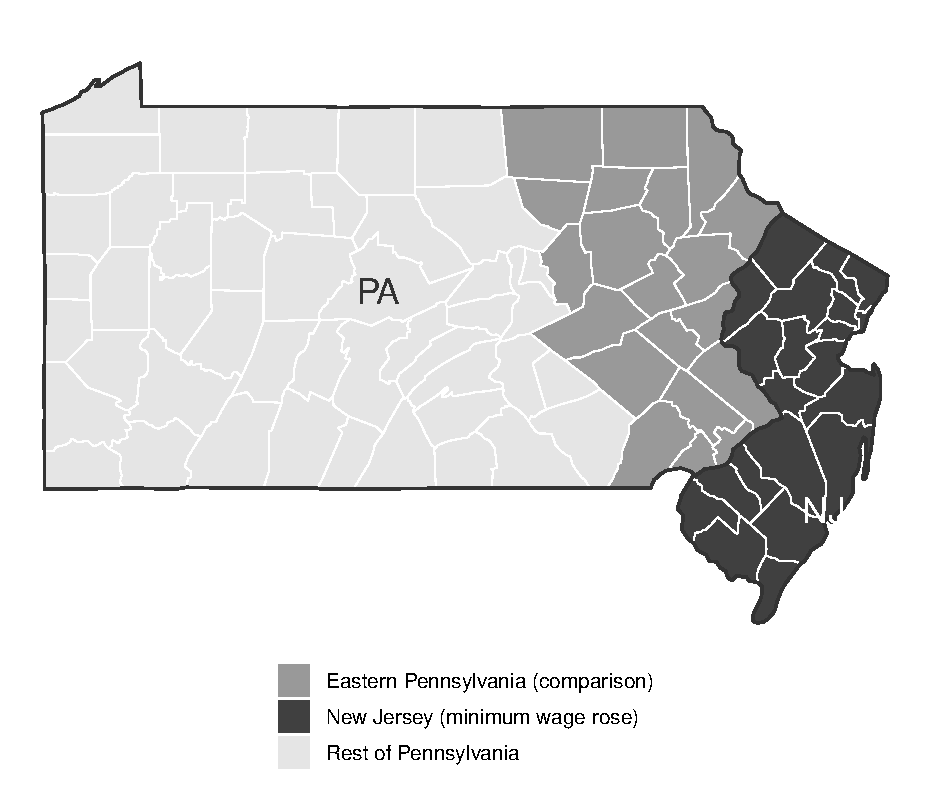
\includegraphics[height=2.45in,keepaspectratio=1]{ck_map_2026.pdf}
\end{center}
\slidesource{Stores were surveyed in New Jersey and in eastern Pennsylvania, on both sides of the border \parencite{card1994minimum}; county boundaries from the \texttt{maps} package.}
\end{frame}


\begin{frame}
  \frametitle{Wages Before \& After Rise in Minimum Wage}
\begin{columns}[T]
\column{.5\textwidth}
\begin{center}
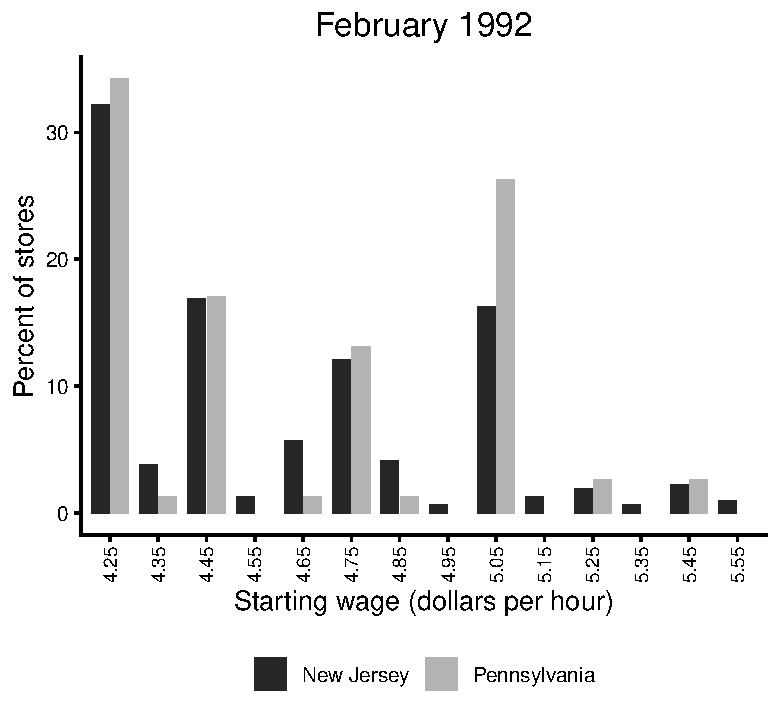
\includegraphics[height=2.3in,keepaspectratio=1]{ck_wages_before_2026.pdf}
\end{center}\pause
\column{.5\textwidth}
\begin{center}
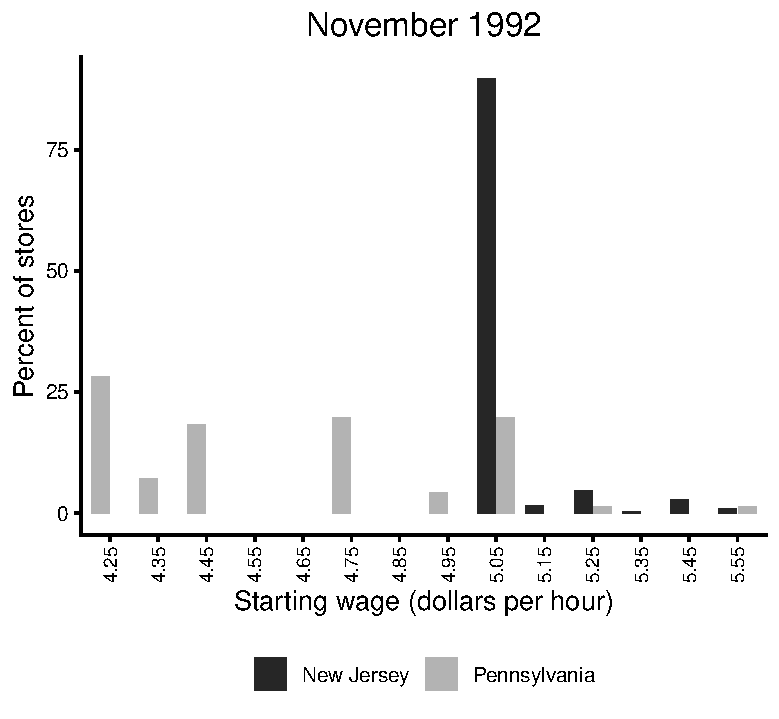
\includegraphics[height=2.3in,keepaspectratio=1]{ck_wages_after_2026.pdf}
\end{center}
\end{columns}
\slidesource{Starting wages in the surveyed stores; own tabulation of the \textcite{card1994minimum} data (\texttt{card\_krueger\_2026.R}).}
\end{frame}


\begin{frame}
 \frametitle{Example: The Mariel Boatlift}
\begin{columns}[c]  
\column{.4\textwidth}
\begin{center}
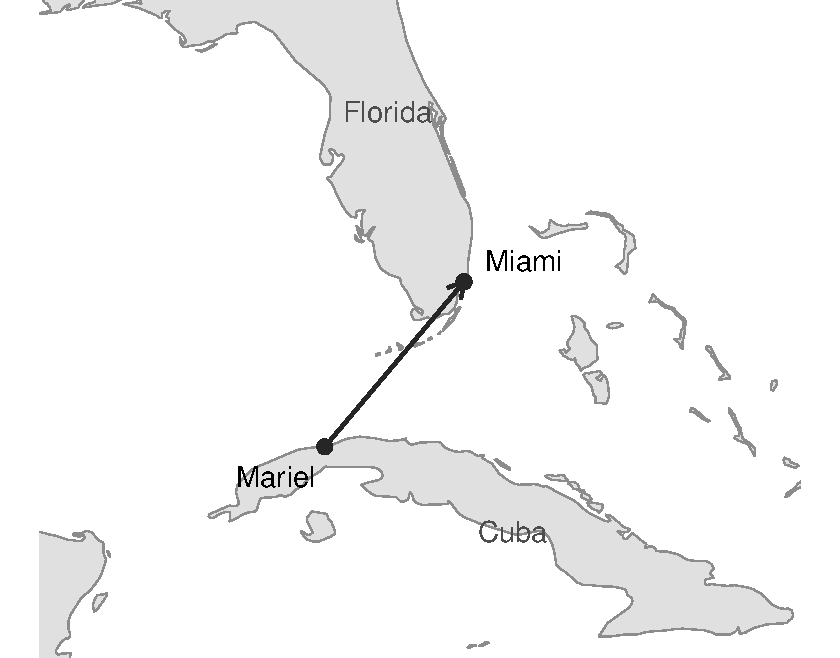
\includegraphics[height=2.3in,keepaspectratio=1]{mariel_map_2026.pdf}
\end{center}\pause
\column{.6\textwidth}
\begin{itemize}[<+->]\itemsep0.5em
\item How do inflows of immigrants affect the wages and employment of natives in local labour markets?
\item \textcite{card1990impact} uses the Mariel Boatlift of 1980 as a natural experiment
to measure the effect of a sudden influx of immigrants on unemployment among less-skilled natives
\item The Mariel Boatlift increased the Miami labor force by 7\%
\item Individual-level data on unemployment from the Current Population Survey (CPS) for Miami and four comparison cities (Atlanta, Los Angeles, Houston and Tampa-St. Petersburg)
\end{itemize}
\end{columns}
\end{frame}


\begin{frame}
  \frametitle{A DID Is a Claim about the Missing Trend}
\begin{center}
\begin{tabular}{lcc}
 & Before the increase & After the increase \\ \hline
New Jersey & observed & \alert{never observed} \\
Pennsylvania & observed & observed \\
\end{tabular}\\[0.5em]
{\small Every cell is $Y_{it}(0)$: employment \emph{without} the increase.}
\end{center}
\bigskip
\keyquestion{Absent the minimum-wage increase, would New Jersey employment have moved like Pennsylvania's?}
\begin{itemize}
\item The comparison can be another state, market, firm, or product.
\item Here, Pennsylvania must be unaffected by New Jersey's law but exposed to the same regional shocks.
\end{itemize}
\end{frame}


\section{Setup \& Identification}


\begin{frame}
  \frametitle{Two Groups and Two Periods}
\begin{Definition}
Two groups:
\begin{itemize}
\item $G=1$ Treated units
\item $G=0$ Control units
\end{itemize}\medskip
Two periods:
\begin{itemize}
\item $t=pre$: Pre-Treatment period
\item $t=pst$: Post-Treatment period
\end{itemize}\medskip
Treatment assignment:
\begin{itemize}
\item $D_{i,t}=1$ if $G_{i} = 1$ and $t = pst$; $D_{i,t}=0$ otherwise
\end{itemize}\medskip
Potential outcomes $Y_{t}(g)$:
\begin{itemize}
\item $Y_{i,t}(1)$ potential outcome unit $i$ attains in period $t$ w/
treatment received between $pre$ and $pst$
\item $Y_{i,t}(0)$ potential outcome unit $i$ attains in period $t$ w/o treatment received between $pre$ and $pst$
\end{itemize}
\end{Definition}
\end{frame}

\begin{frame}
  \frametitle{Two Groups and Two Periods}
\begin{Definition}
Causal effect for unit $i$ at time $t$ is
\begin{itemize}
\item $\tau_{it}=Y_{i,t}(1)-Y_{i,t}(0)$
\end{itemize}\medskip
Observed outcomes $Y_{i,t}$ are realized as
\begin{itemize}
\item $Y_{i,t}=Y_{i,t}(0)\cdot (1-G_{i})+Y_{i,t}(1)\cdot G_{i}$
\end{itemize}\medskip
In the $pst$ period, we have,
\begin{itemize}
  \item  $Y_{i,pst}=Y_{i,pst}(0)\cdot (1-G_i)+Y_{i,pst}(1)\cdot G_i$
\end{itemize}
\end{Definition}
\begin{estm}[ATT]
Focus on estimating the average effect of the treatment on the treated:
$\tau_{ATT}= E[Y_{i,pst}(1)-Y_{i,pst}(0)|G_{i}=1]$
\end{estm}
\end{frame}


\begin{frame}
  \frametitle{Two Groups and Two Periods}
  \begin{estm}[ATT]
$\tau_{ATT}=E[Y_{pst}(1)-Y_{pst}(0)|G=1]$
\end{estm}
\begin{center}
\begin{tabular}{|c|c|c|}
\hline
    {\bf } & {\bf Pre-Period (T=$pre$)} & {\bf Post-Period (T=$pst$)} \\
\hline
\multirow{2}{*}{Treated G=1} & \multirow{2}{*}{\alt<1|handout:0>{$E[Y_{pre}\hphantom{(1)}|G=1]$}{$E[Y_{pre}(1)|G=1]$}} & \multirow{2}{*}{\alt<1|handout:0>{$E[Y_{pst}\hphantom{(1)}|G=1]$}{$E[Y_{pst}(1)|G=1]$}}   \\
 & &  \\
\hline
\multirow{2}{*}{Control G=0} & \multirow{2}{*}{\alt<1|handout:0>{$E[Y_{pre}\hphantom{(0)}|G=0]$}{$E[Y_{pre}(0)|G=0]$}} & \multirow{2}{*}{\alt<1|handout:0>{$E[Y_{pst}\hphantom{(0)}|G=0]$}{$E[Y_{pst}(0)|G=0]$}}   \\
 & &  \\
\hline
\end{tabular}
\end{center}
\begin{overprint}
\onslide<2|handout:1>
\begin{problem}
Missing potential outcome: \textcolor{red}{$E[Y_{pst}(0)|G=1]$}, ie. what is the average post-period outcome for the treated in the absence of the treatment?
\end{problem}
\end{overprint}
\end{frame}


\begin{frame}
  \frametitle{Graphical Representation}
 \setlength{\unitlength}{1cm}
 \hspace*{0.5cm}\begin{picture}(8,6)(-4,-0.5)
 \linethickness{0.5pt}
 \thicklines
 \put(0,0){\vector(1,0){7}}
 \put(0,0){\vector(0,1){5.5}}
 \put(1,0.5){\line(3,1){3.5}}
 \put(1,2){\line(5,3){3.5}}
 \put(1,0.5){\circle*{0.1}}
 \put(1,2){\circle*{0.1}}
 \put(4.5,1.663){\circle*{0.1}}
 \put(4.5,4.1){\circle*{0.1}}
 \put(1,-0.1){\line(0,1){0.2}}
 \put(4.5,-0.1){\line(0,1){0.2}}
 \put(0.6,-0.5){$t=0$}
 \put(4.1,-0.5){$t=1$}
 \thinlines
 \multiput(0,0.5)(0.2,0){5}{\line(1,0){0.1}}
 \multiput(0,2)(0.2,0){5}{\line(1,0){0.1}}
 \multiput(0,1.663)(0.2,0){22}{\line(1,0){0.1}}
 \multiput(0,4.1)(0.2,0){22}{\line(1,0){0.1}}
 \put(-2.5,0.4){\small$E[Y_{pre}(0)|G=0]$}
 \put(-2.5,2){\small$E[Y_{pre}(1)|G=1]$}
 \put(-2.5,1.45){\small$E[Y_{pst}(0)|G=0]$}
 \put(-2.5,4){\small$E[Y_{pst}(1)|G=1]$}
\end{picture}
\end{frame}


\begin{frame}
  \frametitle{Graphical Representation}
 \setlength{\unitlength}{1cm}
 \hspace*{0.5cm}\begin{picture}(8,6)(-4,-0.5)
 \linethickness{0.5pt}
 \thicklines
 \put(0,0){\vector(1,0){7}}
 \put(0,0){\vector(0,1){5.5}}
 \put(1,0.5){\line(3,1){3.5}}
 \put(1,2){\line(5,3){3.5}}
 \put(1,0.5){\circle*{0.1}}
 \put(1,2){\circle*{0.1}}
 \put(4.5,1.663){\circle*{0.1}}
 \put(4.5,4.1){\circle*{0.1}}
 \put(1,-0.1){\line(0,1){0.2}}
 \put(4.5,-0.1){\line(0,1){0.2}}
 \put(0.6,-0.5){$t=0$}
 \put(4.1,-0.5){$t=1$}
 \thinlines
 \multiput(0,0.5)(0.2,0){5}{\line(1,0){0.1}}
 \multiput(0,2)(0.2,0){5}{\line(1,0){0.1}}
 \multiput(0,1.663)(0.2,0){22}{\line(1,0){0.1}}
 \multiput(0,4.1)(0.2,0){22}{\line(1,0){0.1}}
 \put(-2.5,0.4){\small$E[Y_{pre}(0)|G=0]$}
 \put(-2.5,2){\small\red{$E[Y_{pre}(0)|G=1]$}}
 \put(-2.5,1.45){\small$E[Y_{pst}(0)|G=0]$}
 \put(-2.5,4){\small$E[Y_{pst}(1)|G=1]$}
\end{picture}
\end{frame}

\begin{frame}
  \frametitle{Graphical Representation}
 \setlength{\unitlength}{1cm}
 \hspace*{0.5cm}\begin{picture}(8,6)(-4,-0.5)
 \linethickness{0.5pt}
 \thicklines
 \put(0,0){\vector(1,0){7}}
 \put(0,0){\vector(0,1){5.5}}
 \put(1,0.5){\line(3,1){3.5}}
 \put(1,2){\line(5,3){3.5}}
 \put(1,0.5){\circle*{0.1}}
 \put(1,2){\circle*{0.1}}
 \put(4.5,1.663){\circle*{0.1}}
 \put(4.5,4.1){\circle*{0.1}}
 \put(1,-0.1){\line(0,1){0.2}}
 \put(4.5,-0.1){\line(0,1){0.2}}
 \put(0.6,-0.5){$t=0$}
 \put(4.1,-0.5){$t=1$}
 \thinlines
 \multiput(0,0.5)(0.2,0){5}{\line(1,0){0.1}}
 \multiput(0,2)(0.2,0){5}{\line(1,0){0.1}}
 \multiput(0,1.663)(0.2,0){22}{\line(1,0){0.1}}
 \multiput(0,4.1)(0.2,0){22}{\line(1,0){0.1}}
 \put(-2.5,0.4){\small$E[Y_{pre}(0)|G=0]$}
 \put(-2.5,2){\small\red{$E[Y_{pre}(0)|G=1]$}}
 \put(-2.5,1.45){\small$E[Y_{pst}(0)|G=0]$}
 \put(-2.5,4){\small$E[Y_{pst}(1)|G=1]$}
 \multiput(1,2)(0.6,0.2){6}{\line(3,1){0.4}}
 \put(4.5,3.163){\circle{0.1}}
 \multiput(0,3.163)(0.2,0){22}{\line(1,0){0.1}}
 \put(-2.5,3.1){\small\red{$E[Y_{pst}(0)|G=1]$}}
 \onslide<2-> \thicklines
 \put(4.5,3.25){\vector(0,1){0.8}}
 \put(4.5,4){\vector(0,-1){0.75}}
 \put(4.7,3.5){\small $E[Y_{pst}(1)-Y_{pst}(0)|G=1]$}
\end{picture}
\end{frame}


\begin{frame}
  \frametitle{DID: Identification}
\begin{iass}[no anticipation]\small
    $$Y_{i,pre}(0) = Y_{pre}(1), i = 1, 2, \cdots, n$$
\end{iass}  
\begin{iass}[parallel trends]\small
$$E[Y_{pst}(0)-Y_{pre}(0)|G=1]=E[Y_{pst}(0)-Y_{pre}(0)|G=0]$$
\end{iass}
\begin{overprint}
\onslide<1|handout:1>
\begin{ires}\small
Given no anticipation and parallel trends, the ATT is identified as:
\begin{equation*}
E[Y_{pst}(1)-Y_{pst}(0)|G=1]=\Bigl\{ E[Y_{pst}|G=1]-E[Y_{pst}|G=0] \Bigr\} -\Bigl\{ E[Y_{pre}|G=1]-E[Y_{pre}|G=0] \Bigr\}
\end{equation*}
\end{ires}
\onslide<2|handout:2>
\scriptsize\vspace{-0.5cm}
\begin{Proof}
Plug in $\red{E[Y_{pre}(1)|G=1] = E[Y_{pre}(0)|G=1]}$ and $\alert{E[Y_{pst}(0)|G=0]} = E[Y_{pst}(0)|G=1] - E[Y_{pre}(0)|G=1] + E[Y_{pre}(0)|G=0]$\\
we get
\begin{eqnarray*}
% \nonumber to remove numbering (before each equation)
  \tau_{DID} & \equiv & \left\{ E[Y_{pst}|G=1]-E[Y_{pst}|G=0] \right\}
      -\left\{ E[Y_{pre}|G=1]-E[Y_{pre}|G=0] \right\}\\
   &=&  \left\{ E[Y_{pst}(1)|G=1]-\alert{E[Y_{pst}(0)|G=0]} \right\}
      -\left\{ \red{E[Y_{pre}(0)|G=1]}-E[Y_{pre}(0)|G=0] \right\} \\    
&=& \left\{ E[Y_{pst}(1)|G=1]- \left( E[Y_{pst}(0)|G=1] - E[Y_{pre}(0)|G=1] + E[Y_{pre}(0)|G=0] \right) \right\} \\
&-& \left\{ E[Y_{pre}(0)|G=1]-E[Y_{pre}(0)|G=0] \right\}\\
&=&E[Y_{pst}(1)-Y_{pst}(0)|G=1]
\end{eqnarray*}
\end{Proof}
\end{overprint}
\end{frame}


\section{DID Estimation}

\begin{frame}
  \frametitle{DID: Estimators}
\begin{estm}[Identifying the ATT]\small
$$\tau_{DID} = E[Y_{pst}(1)-Y_{pst}(0)|G=1]$$\pause
\end{estm}\vspace{-.05in}
\begin{esti}[Sample Means: Panel]\small
\[
  \hat\tau_{DID} = \left\{\frac{1}{N_1}\sum_{G_i=1} Y_{i,pst} -
\frac{1}{N_0}\sum_{G_i=0} Y_{i,pst}\right\} -
\left\{\frac{1}{N_1}\sum_{G_i=1} Y_{i,pre} -
\frac{1}{N_0}\sum_{G_i=0} Y_{i,pre}\right\}
\]
\[
=\left\{\frac{1}{N_1}\sum_{G_i=1} \{Y_i(1)-Y_{i,pre}\} -
\frac{1}{N_0}\sum_{G_i=0} \{Y_i(1)-Y_{i,pre}\}\right\},
\]
where $N_1$ and $N_0$ are the number of treated and control units respectively, and
$$\operatorname{plim} \hat\tau_{DID} = \tau_{DID}$$
\end{esti}
\end{frame}

\begin{frame}
  \frametitle{Sample Means: Minimum Wage Laws and Employment}
\begin{columns}[T,onlytextwidth]
\begin{column}{0.43\textwidth}
\centering
\small
\renewcommand{\arraystretch}{1.35}
\begin{tabular}{lccc}
\hline
FTE employment & PA & NJ & NJ$-$PA \\ \hline
Before  & 23.33 & 20.44 & $-2.89$ \\
After   & 21.17 & 21.03 & $-0.14$ \\ \hline
Change  & $-2.16$ & $0.59$ & \alert{\bfseries 2.76} \\ \hline
\end{tabular}
\end{column}
\begin{column}{0.55\textwidth}
\centering
\begin{tikzpicture}[font=\scriptsize]
  \draw[SlideInk!45] (0,0) -- (0,3.7);
  \draw[SlideInk!45] (0,0) -- (3.9,0);
  \foreach \v/\y in {19/0.6, 21/1.8, 23/3.0}{%
    \draw[SlideInk!45] (-0.08,\y) -- (0,\y);
    \node[left, text=SlideInk!70, inner sep=1.5pt] at (-0.08,\y) {\v};}
  \node[rotate=90, text=SlideInk!70, font=\tiny] at (-0.82,1.85) {FTE employment per store};
  \node[below, text=SlideInk!70] at (0.6,0) {Before};
  \node[below, text=SlideInk!70] at (3.4,0) {After};
  % Pennsylvania
  \draw[SlideBlue, very thick] (0.6,3.20) -- (3.4,1.90);
  \fill[SlideBlue] (0.6,3.20) circle (1.7pt) (3.4,1.90) circle (1.7pt);
  \node[above, text=SlideBlue] at (2.0,2.55) {PA};
  % New Jersey, observed
  \draw[SlideRed, very thick] (0.6,1.46) -- (3.4,1.82);
  \fill[SlideRed] (0.6,1.46) circle (1.7pt) (3.4,1.82) circle (1.7pt);
  \node[above, text=SlideRed] at (2.0,1.64) {NJ};
  % New Jersey, if it had moved like Pennsylvania
  \draw[SlideRed!50, very thick, dashed] (0.6,1.46) -- (3.4,0.17)
    node[sloped, midway, below, text=SlideRed!75, font=\tiny] {NJ counterfactual};
  \draw[SlideRed!50, fill=white, thick] (3.4,0.17) circle (1.7pt);
  % the difference-in-differences
  \draw[{Latex[length=1.4mm]}-{Latex[length=1.4mm]}, SlideInk] (3.6,0.17) -- (3.6,1.82);
  \node[right, text=SlideInk] at (3.62,1.0) {$\hat\tau_{DID}=2.76$};
\end{tikzpicture}
\end{column}
\end{columns}
\slidesource{\textcite{card1994minimum}, Table 3, rows 1--3.}
\end{frame}

\begin{frame}
  \frametitle{Sample Means: The Mariel Boatlift}
\begin{columns}[T,onlytextwidth]
\begin{column}{0.44\textwidth}
\centering
\scriptsize
\renewcommand{\arraystretch}{1.2}
\begin{tabular}{lcccc}
\hline
 & \multicolumn{2}{c}{Mean log wage} & \multicolumn{2}{c}{Miami $-$ outside} \\
 & Miami & Outside & Unadj. & Adj. \\ \hline
1979 & 1.58 & 1.71 & \alert{$-.13$} & \alert{$-.10$} \\
1980 & 1.54 & 1.66 & $-.12$ & $-.06$ \\
1981 & 1.51 & 1.63 & $-.13$ & $-.09$ \\
1982 & 1.49 & 1.71 & $-.22$ & $-.12$ \\
1983 & 1.48 & 1.62 & $-.14$ & $-.08$ \\
1984 & 1.53 & 1.63 & $-.10$ & $-.08$ \\
1985 & 1.49 & 1.77 & $-.27$ & $-.19$ \\ \hline
\end{tabular}\\[0.4em]
{\tiny Cubans in Miami vs.\ Cubans elsewhere; 1979 is the last full pre-boatlift\\
year. Adjusted controls for education, potential experience, gender, marital\\
status, part-time status, and public vs.\ private sector.}
\end{column}
\begin{column}{0.54\textwidth}
\centering
\begin{tikzpicture}[font=\scriptsize]
  \draw[SlideInk!45] (-0.15,1.0) -- (-0.15,3.8);
  \draw[SlideInk!45] (-0.15,1.0) -- (4.35,1.0);
  \foreach \v/\y in {{$-.3$}/1.12, {$-.2$}/1.92, {$-.1$}/2.72, {$0$}/3.52}{%
    \draw[SlideInk!45] (-0.23,\y) -- (-0.15,\y);
    \node[left, text=SlideInk!70, font=\tiny, inner sep=1.5pt] at (-0.23,\y) {\v};}
  \node[rotate=90, text=SlideInk!70, font=\tiny] at (-0.95,2.4)
    {Log wage gap (Miami $-$ rest of U.S.)};
  \foreach \t/\x in {{'79}/0, {'80}/0.68, {'81}/1.36, {'82}/2.04, {'83}/2.72, {'84}/3.40, {'85}/4.08}
    {\node[below, text=SlideInk!70, font=\tiny] at (\x,1.0) {\t};}
  % no-gap reference
  \draw[SlideInk!30, dotted] (-0.15,3.52) -- (4.25,3.52);
  % the boatlift arrived mid-1980
  \draw[SlideInk!35, dashed] (1.02,1.0) -- (1.02,3.68);
  \node[above, text=SlideInk!60, font=\tiny] at (1.02,3.68) {boatlift};
  % adjusted difference
  \draw[SlideBlue, very thick]
    (0,2.72) -- (0.68,3.04) -- (1.36,2.80) -- (2.04,2.56) -- (2.72,2.88) -- (3.40,2.88) -- (4.08,2.00);
  \foreach \x/\y in {0/2.72, 0.68/3.04, 1.36/2.80, 2.04/2.56, 2.72/2.88, 3.40/2.88, 4.08/2.00}
    {\fill[SlideBlue] (\x,\y) circle (1.5pt);}
  \node[right, text=SlideBlue, font=\tiny] at (4.13,2.00) {adjusted};
  % unadjusted difference
  \draw[SlideRed, very thick]
    (0,2.48) -- (0.68,2.56) -- (1.36,2.48) -- (2.04,1.76) -- (2.72,2.40) -- (3.40,2.72) -- (4.08,1.36);
  \foreach \x/\y in {0/2.48, 0.68/2.56, 1.36/2.48, 2.04/1.76, 2.72/2.40, 3.40/2.72, 4.08/1.36}
    {\fill[SlideRed] (\x,\y) circle (1.5pt);}
  \node[right, text=SlideRed, font=\tiny] at (4.13,1.36) {unadjusted};
\end{tikzpicture}
\end{column}
\end{columns}
\slidesource{\textcite{card1990impact}, Table 7; the two difference columns are his ninth and tenth.}
\end{frame}


% \footnotesize
% \begin{lstlisting}[language=R, basicstyle=\ttfamily]
% with(d, 
%  (
%   mean(emptot[nj == 1 & postperiod == 1], na.rm = TRUE) - 
%   mean(emptot[nj == 1 & postperiod == 0], na.rm = TRUE)
%   )  - 
%   (mean(emptot[nj == 0 & postperiod == 1], na.rm = TRUE) - 
%   mean(emptot[nj == 0 & postperiod == 0], na.rm = TRUE)
%   )
%  )
% [1] 2.753606
% \end{lstlisting}

% \end{frame}


% t test of coefficients:

%               Estimate Std. Error t value Pr(>|t|)    
% (Intercept)    23.3312     1.0719 21.7668  < 2e-16 ***
% postperiod     -2.1656     1.5159 -1.4286  0.15351    
% nj             -2.8918     1.1935 -2.4229  0.01562 *  
% postperiod:nj   2.7536     1.6884  1.6309  0.10331    
% \end{verbatim}
% Note: Should adjust standard errors to account for temporal dependence
% \end{frame}


\begin{frame}
  \frametitle{DID: Estimators}
\begin{esti}[Regression: Panel Data]\small
With panel data we can estimate the difference-in-differences effect using a fixed effects regression with unit and  period fixed effects:
\[
Y_{it} = \mu + \gamma_i + \delta T + \tau D_{it} + X'_{it}\beta + \varepsilon_{it}
\]\vspace*{-0.5cm}

\begin{itemize}
\item One intercept for each unit $\gamma_i$
\item $D_{it}$ coded as 1 for treated in post-period and 0 otherwise
%\item Correct standard errors to account for temporal dependence
\end{itemize}

Or equivalently we can use regression with the dependent variable in first differences:
\[
\Delta Y_i = \delta + \tau \cdot G_i + u_i,
\]
where $\Delta Y_i = Y_i(1)-Y_{i,pre}$ and $u_i=\Delta \varepsilon_i$.\\\bigskip
\end{esti}
\end{frame}


% > d$Dit <- d$nj * d$postperiod

% > d <- plm.data(d, indexes = c("ID", "postperiod"))

% > did.reg <- plm(emptot ~ postperiod + Dit, data = d,
%                           model = "within")

% > coeftest(did.reg, vcov=function(x) 
%                  vcovHC(x, cluster="group", type="HC1"))

% t test of coefficients:


% t test of coefficients:


\begin{frame}[fragile]
  \frametitle{R Demo: Card--Krueger in One Regression}
\begin{lstlisting}[language=R]
library(haven)
library(fixest)

ck <- read_dta("figs/CK1994_longformat.dta")
m <- feols(emptot ~ nj * postperiod | ID,
           data = ck, cluster = ~ID)
etable(m)
\end{lstlisting}
\begin{center}
\begin{tabular}{lrr}
 & Estimate & Clustered SE \\ \hline
NJ $\times$ post & 2.750 & 1.338 \\
\end{tabular}
\end{center}
The interaction coefficient is the DID estimate.
\end{frame}

\begin{frame}
  \frametitle{IPW (reweighting) + DID}
  \begin{itemize}\itemsep1em
\item \textbf{Assumption}: non-parallel outcome dynamics between treated and
controls caused by observed characteristics, or \red{conditional parallel trends}\pause
    \item \textcite{abadie2005semiparametric} proposes a two-step strategy:
    \begin{enumerate}
      \item estimate the propensity score based on observed covariates; compute the fitted value
      \item run a weighted DID model 
    \end{enumerate}\pause
    \item $\tau_{IPW} = \E\left\{\frac{G_i\cdot \Delta Y_{i}  }{\pi(X_i)} \right\} - \E\left\{\frac{(1-G_i)\cdot \Delta Y_{i}  }{1-\pi(X_i)} \right\}$\pause
    \item The idea of using pre-treatment variables to adjust trends is a precursor to synthetic control\pause
  \item Balancing is an alternative reweighting strategy and has better finite sample
properties   
  \end{itemize}
  \end{frame}


  \begin{frame}{Balancing + DID}
    \begin{itemize}
      \itemsep1.5em
    \item \underline{Mean balancing}: on original features {\small\alert{\parenciteshort{robbins2017framework}}}\\
    \begin{center}
    $\sum_{i\in\T} q_{i}\bY_{i,pre} =\sum_{j\in\C} w_{j}\bY_{j, pre}$
    \end{center}\pause
  \item \underline{Trajectory balancing}: feature mapping  $\bY_{i,pre} \mapsto \phi(\bY_{i,pre})$, then balance on the expanded features {\small\alert{\parencite{hazlett2018trajectory}}}:
    \begin{center}
    $\phi: \mathbb{R}^P \mapsto \mathbb{R}^{P'}$\\
    $\sum_{i\in\T} q_{i}\phi(\bY_{i, pre}) = \sum_{j\in\C} w_{j} \phi(\bY_{j,pre})$
    \end{center}\pause
    \item In practice: seek approximate balance, working from largest toward smallest \red{principal components} of $\bY_{pre}(\bY_{pre})'$ with a stopping rule of minimizing the upper bound of biases
  \end{itemize}
  \end{frame}
  
  
\section{Threats to Validity}

\if\handout1
\begin{frame}
  \frametitle{This Lecture}
\begin{itemize}\itemsep1em
\item Motivating Examples
\item DID: Setup \& Identification
\item DID: Estimation
\item DID: Extensions
\item \textbf{Threats to Validity}
\end{itemize}
\end{frame}
\fi


\begin{frame}
  \frametitle{Threats to Validity}

\begin{enumerate}[<+->]\itemsep0.5em
% \item \emph{Compositional differences}: In repeated cross-sections
%       we do not want that the composition
%       of the sample changes between periods.
% \begin{itemize}
% \item Falsification Test: Distribution of $(D,X)$ should be similar for the pre-treatment and
%       post-treatment periods.
% \end{itemize}\bigskip
\item Non-parallel dynamics
\item Compositional differences
\item Long-term effects versus reliability
\item Scale dependence
\item Staggered adoption: heterogeneous treatment effects \& the weighting problem ($\rightarrow$ Lecture 4)
\end{enumerate}\bigskip\pause
Bias is a matter of degree. Small violations of the identification assumptions may not matter much as the bias may be rather small. However, biases can sometimes be so large that the estimates we get are completely wrong, even of the opposite sign of the true treatment effect.\\\bigskip\pause

Helpful to avoid overly strong causal claims for difference-in-differences estimates.
\end{frame}


\begin{frame}
  \frametitle{Non-parallel Dynamics}
Often treatments/programs are targeted based on pre-existing differences in outcomes.  ``Feedback'' or time-varying confounding cause failure of the parallel trends assumption.\bigskip\pause
% \item \emph{Compositional differences}: In repeated cross-sections
%       we do not want that the composition
%       of the sample changes between periods.
% \begin{itemize}
% \item Falsification Test: Distribution of $(D,X)$ should be similar for the pre-treatment and
%       post-treatment periods.
% \end{itemize}\bigskip
\begin{itemize}[<+->]\itemsep0.5em
   \item ``Ashenfelter dip'': participants in training programs often experience a dip in earnings
just before they enter the program (that may be \emph{why} they participate). Since wages have a natural tendency to mean reversion, comparing wages of participants and non-participants using DD leads to an upward biased estimate of the program effect
   \item Regional targeting: NGOs may target villages that appear most promising (or worst off)
\end{itemize}
\end{frame}

\begin{frame}
  \frametitle{The Ashenfelter Dip}
\begin{columns}[T,onlytextwidth]
\begin{column}{0.60\textwidth}
\centering
\begin{tikzpicture}[font=\scriptsize]
  \draw[SlideInk!45] (-0.15,0) -- (-0.15,4.15);
  \draw[SlideInk!45] (-0.15,0) -- (5.05,0);
  \node[rotate=90, text=SlideInk!70, font=\tiny] at (-0.45,2.1) {Earnings};
  \foreach \t/\x in {{$-3$}/0, {$-2$}/0.95, {$-1$}/1.9, {$0$}/2.85, {$1$}/3.8, {$2$}/4.75}
    {\node[below, text=SlideInk!70] at (\x,0) {\t};}
  \node[text=SlideInk!70, font=\tiny] at (2.4,-0.5) {Period relative to entry};
  % entry into the program
  \draw[SlideInk!35, dashed] (2.85,0) -- (2.85,4.0);
  \node[above, text=SlideInk!60, font=\tiny] at (2.85,4.0) {enters program};
  % non-participants
  \draw[SlideBlue, very thick]
    (0,2.8) -- (0.95,3.0) -- (1.9,3.2) -- (2.85,3.4) -- (3.8,3.6) -- (4.75,3.8);
  \foreach \x/\y in {0/2.8, 0.95/3.0, 1.9/3.2, 2.85/3.4, 3.8/3.6, 4.75/3.8}
    {\fill[SlideBlue] (\x,\y) circle (1.5pt);}
  \node[right, text=SlideBlue, font=\tiny] at (4.8,3.8) {non-participants};
  % participants
  \draw[SlideRed, very thick]
    (0,2.2) -- (0.95,2.3) -- (1.9,0.6) -- (2.85,1.7) -- (3.8,2.7) -- (4.75,3.0);
  \foreach \x/\y in {0/2.2, 0.95/2.3, 1.9/0.6, 2.85/1.7, 3.8/2.7, 4.75/3.0}
    {\fill[SlideRed] (\x,\y) circle (1.5pt);}
  \node[right, text=SlideRed, font=\tiny] at (4.8,2.9) {participants};
  % the dip
  \draw[-{Latex[length=1.4mm]}, SlideInk!80] (1.05,0.22) -- (1.78,0.53);
  \node[left, text=SlideInk, font=\tiny] at (1.05,0.22) {the dip};
\end{tikzpicture}
\end{column}
\begin{column}{0.38\textwidth}
\begin{block}{What happens}
Earnings fall just before entry, which is often \emph{why} people enter, then recover on their own.
\end{block}
\begin{block}{Why DID is biased}
Using $t=-1$ as the baseline counts ordinary recovery as program effect, so the estimate is too large.
\end{block}
\end{column}
\end{columns}

\end{frame}


\begin{frame}
  \frametitle{Falsification Test using Data from Pretreatment Periods}
  \vspace{-.2in}
\begin{center}
  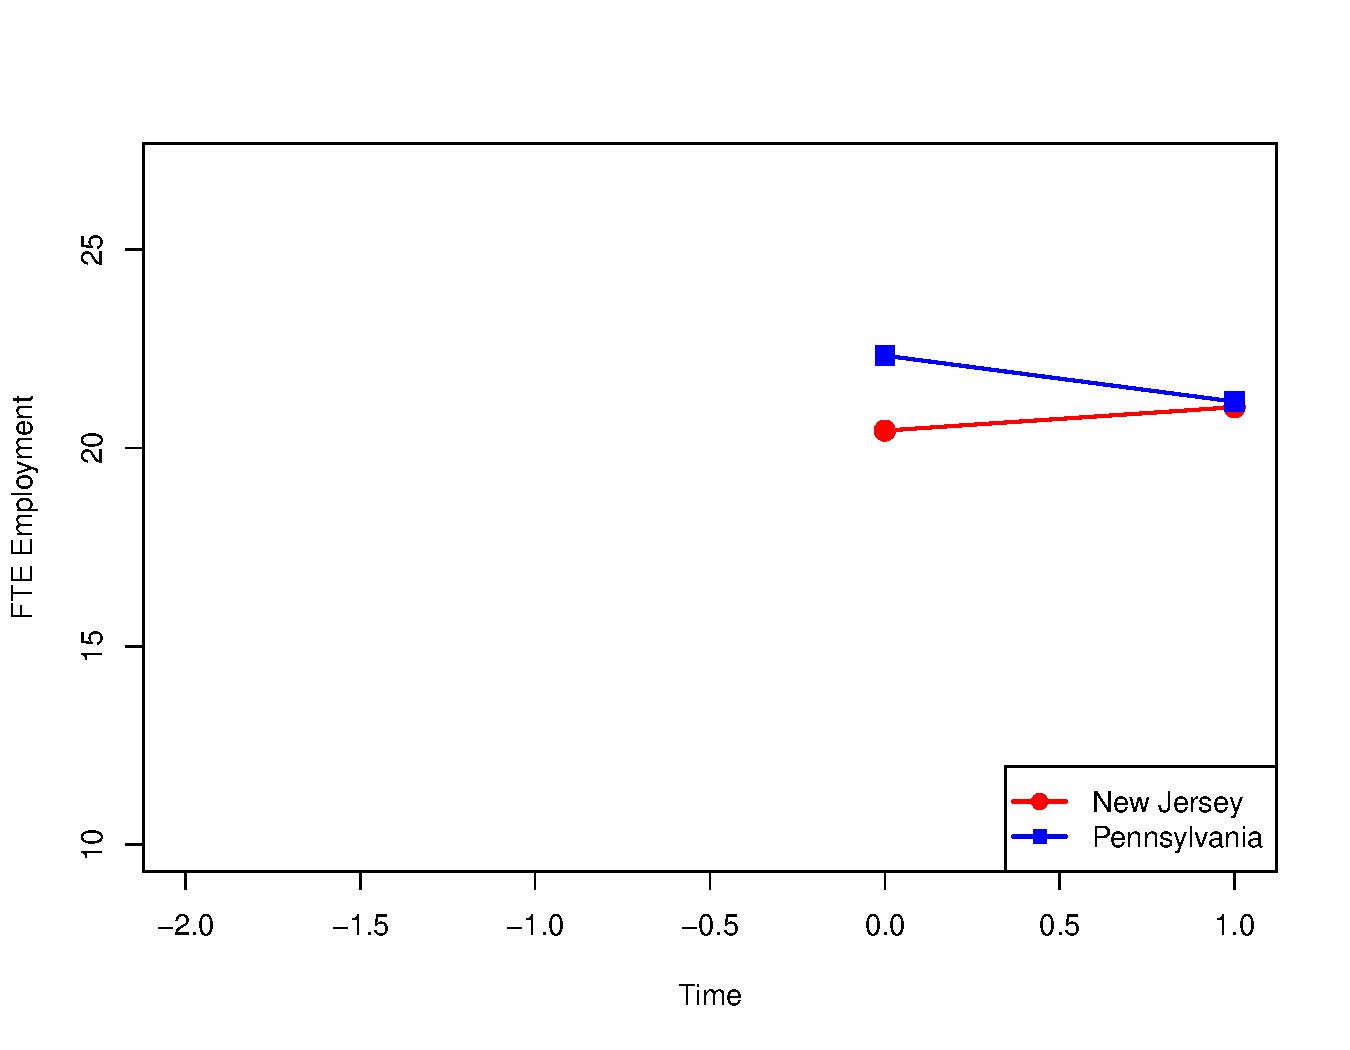
\includegraphics[height=3.2in,keepaspectratio=1]{KCfalsification1.pdf}
\end{center}
\end{frame}

\begin{frame}
  \frametitle{Falsification Test using Data from Pretreatment Periods}
  \vspace{-.2in}
\begin{center}
  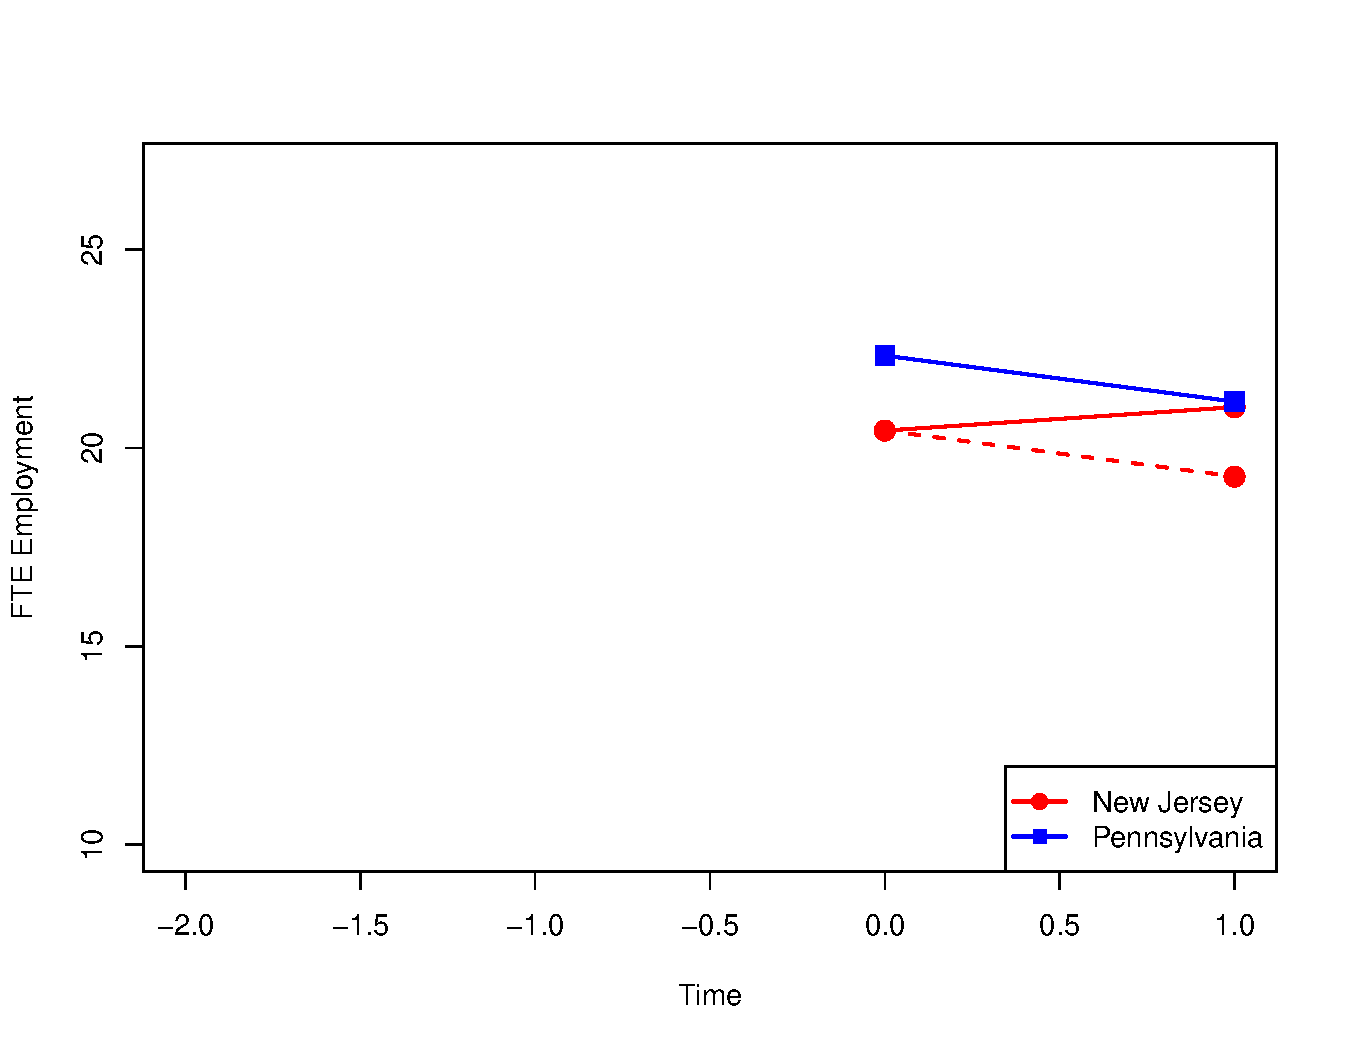
\includegraphics[height=3.2in,keepaspectratio=1]{KCfalsification2.pdf}
\end{center}
\end{frame}

\begin{frame}
  \frametitle{Falsification Test using Data from Pretreatment Periods}
  \vspace{-.2in}
\begin{center}
  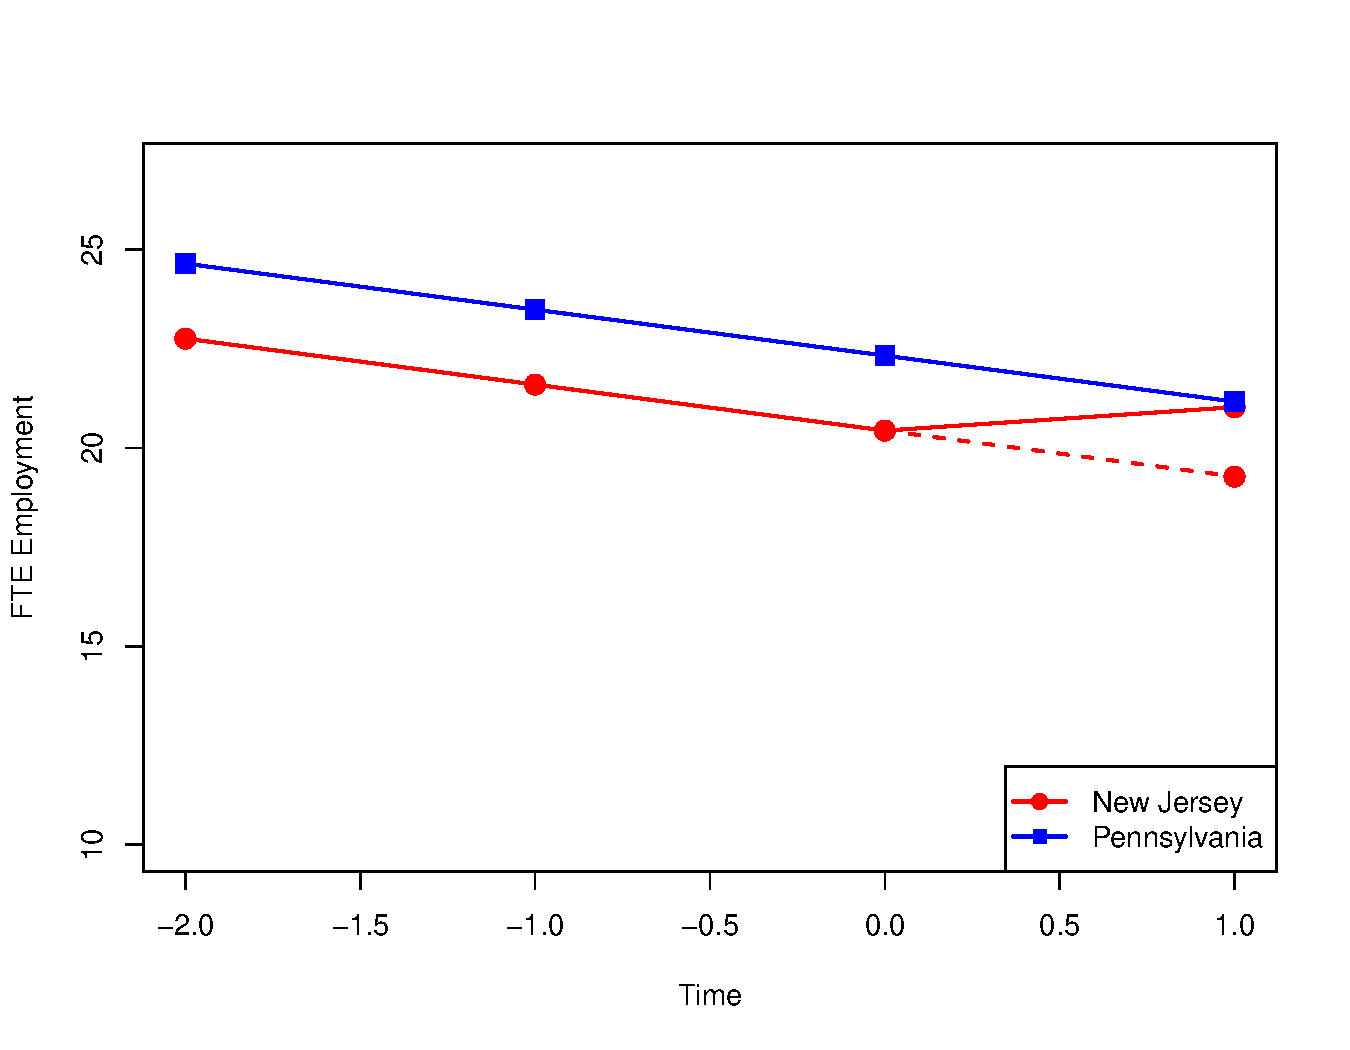
\includegraphics[height=3.2in,keepaspectratio=1]{KCfalsification3.pdf}
\end{center}
\end{frame}

\begin{frame}
  \frametitle{Falsification Test using Data from Pretreatment Periods}
  \vspace{-.2in}
\begin{center}
  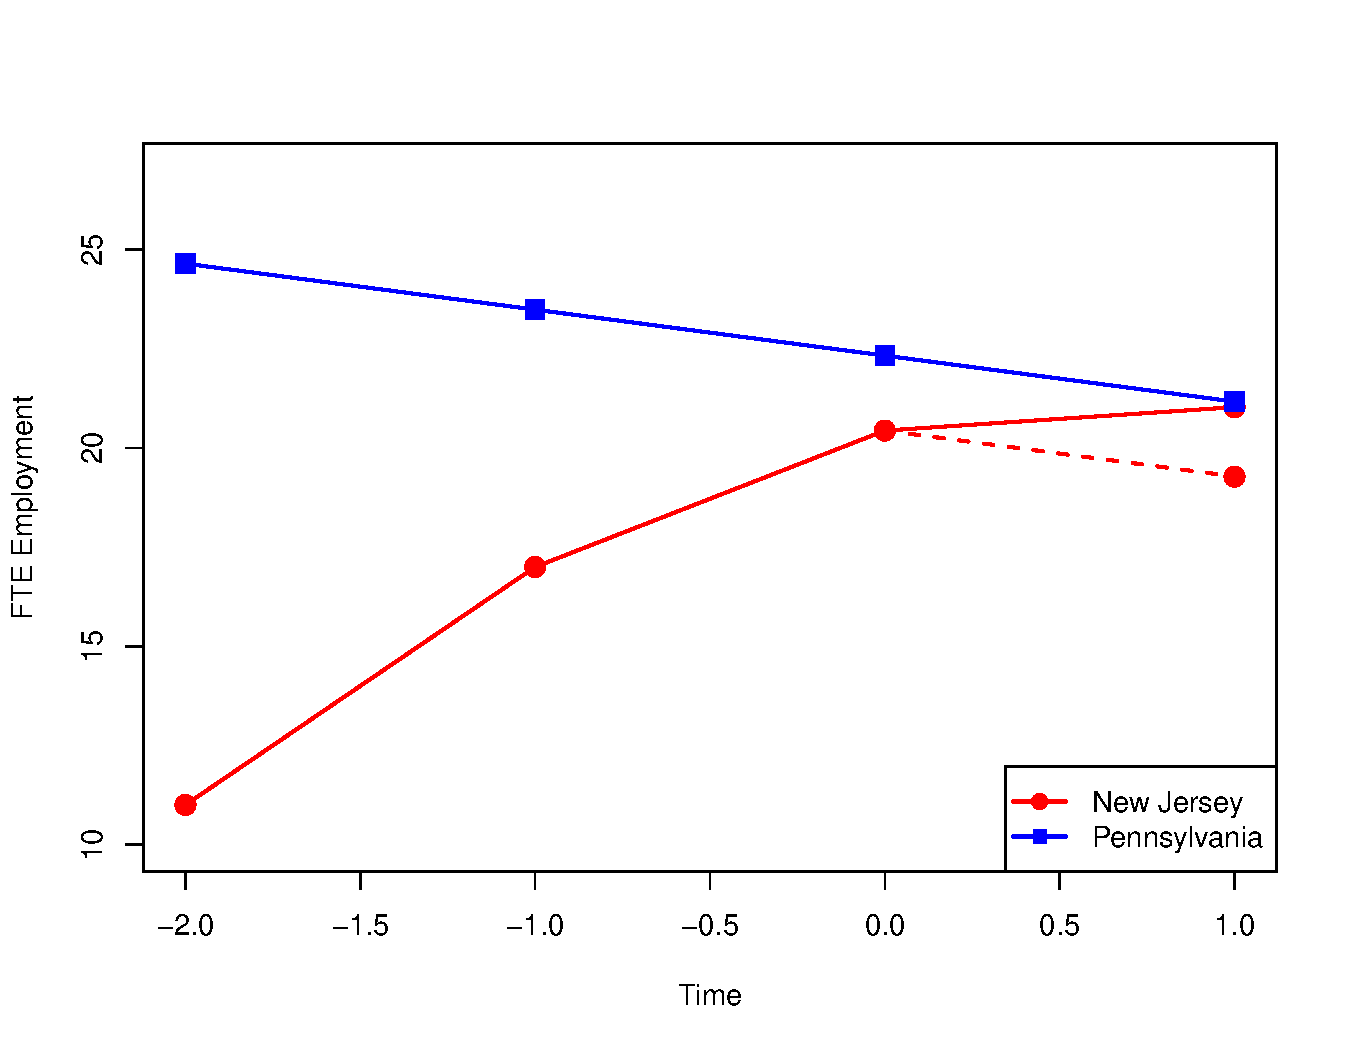
\includegraphics[height=3.2in,keepaspectratio=1]{KCfalsification4.pdf}
\end{center}
\end{frame}

\begin{frame}
  \frametitle{Longer Trends in Employment (\cite{card2000minimum})}
  \vspace{-.1in}
\begin{center}
  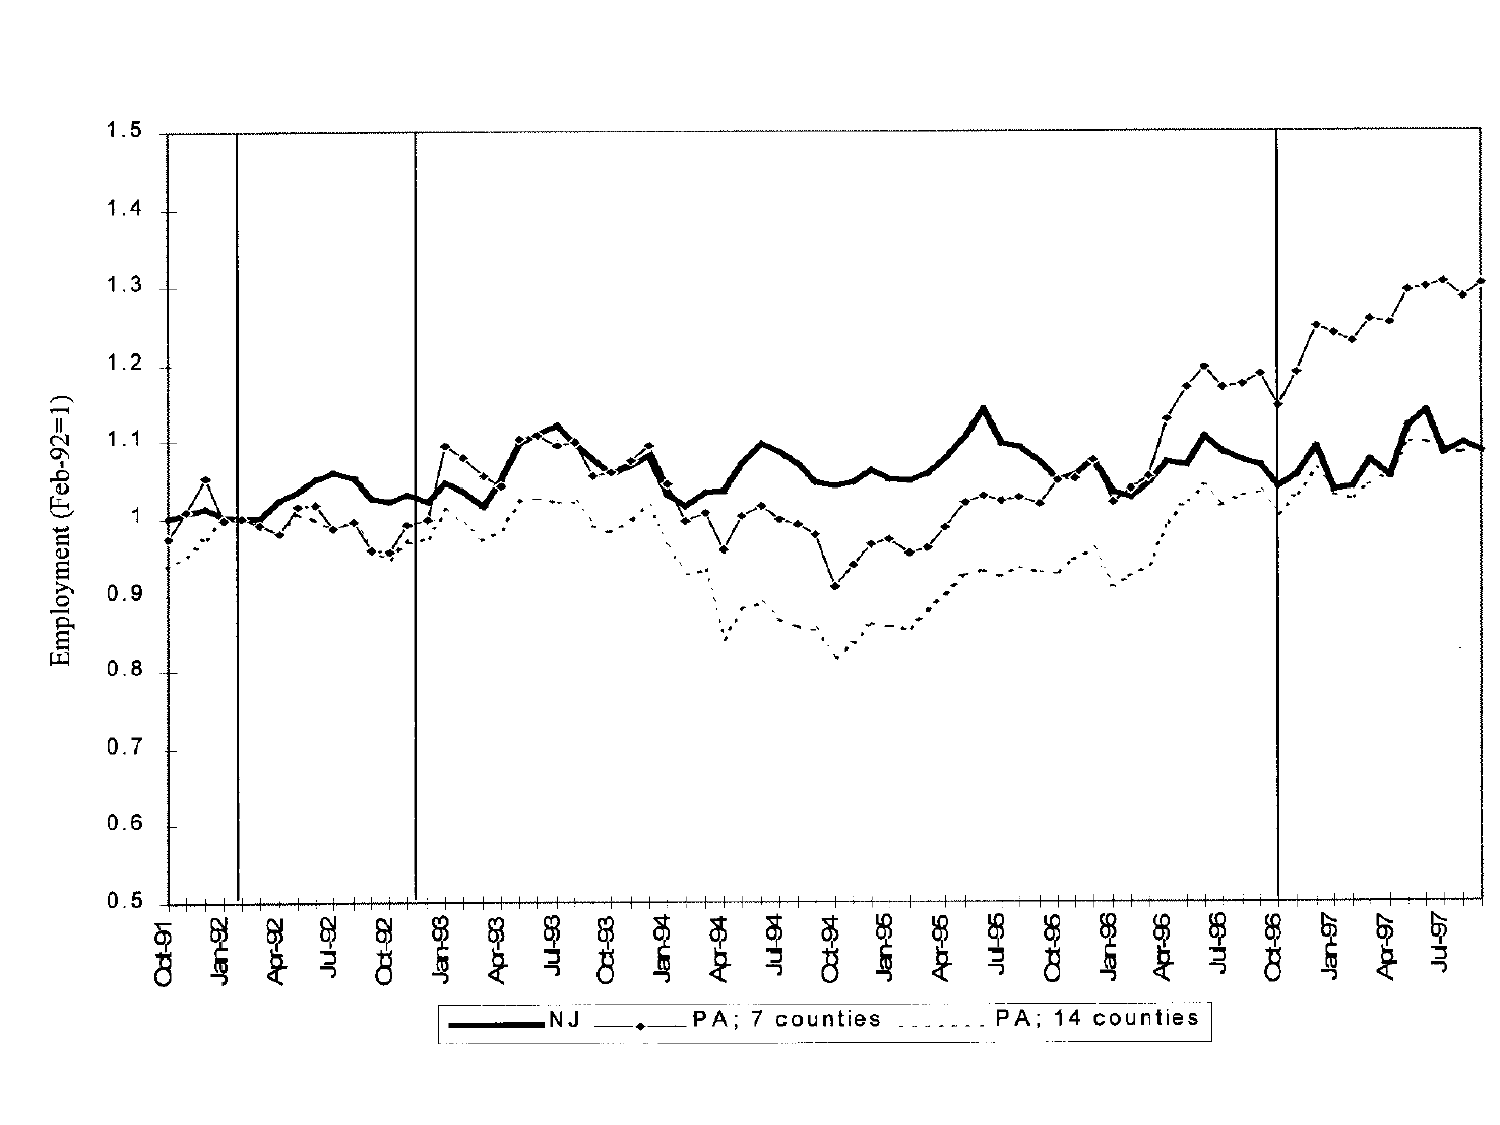
\includegraphics[height=2.6in,keepaspectratio=1]{PreTrend.pdf}
\end{center}
\slidesource{Figure 2 of \textcite{card2000minimum}, reproduced with attribution: employment in eating and drinking places (BLS ES-202), New Jersey and Pennsylvania counties.}
\end{frame}

\begin{frame}[c]
\frametitle{Signs of Parallel Trends Violations}
\bigskip
\begin{columns}
\column{.5\textwidth}
\centering 
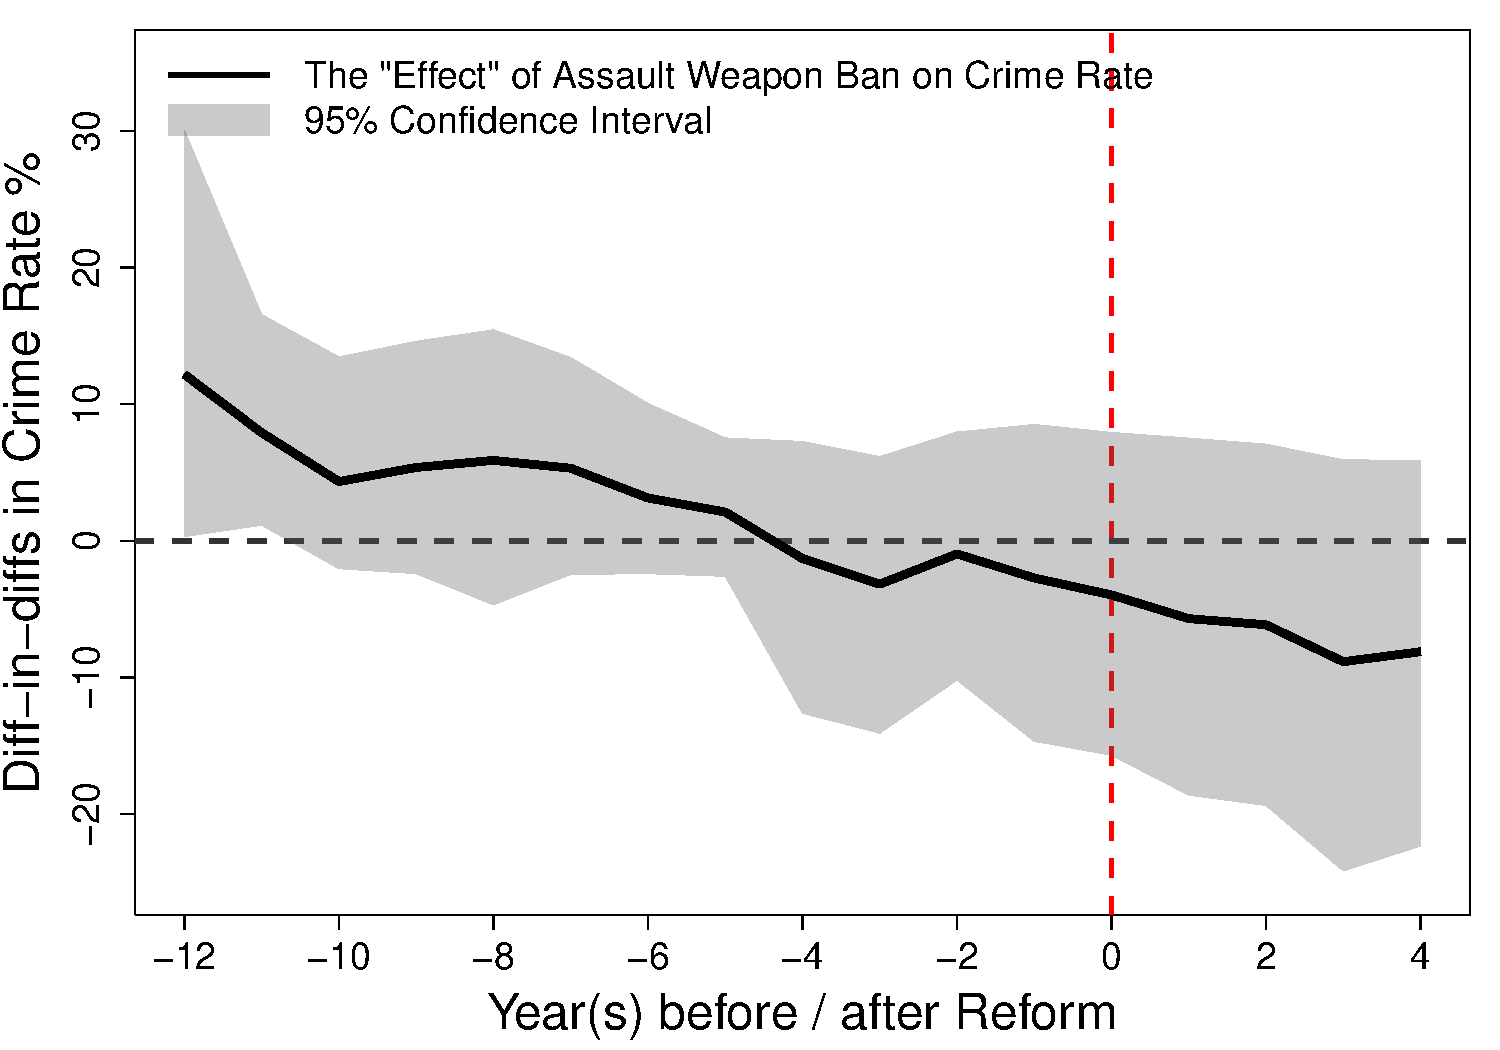
\includegraphics[width=5cm]{ex_guncontrol.pdf}\\\vspace{1em}%
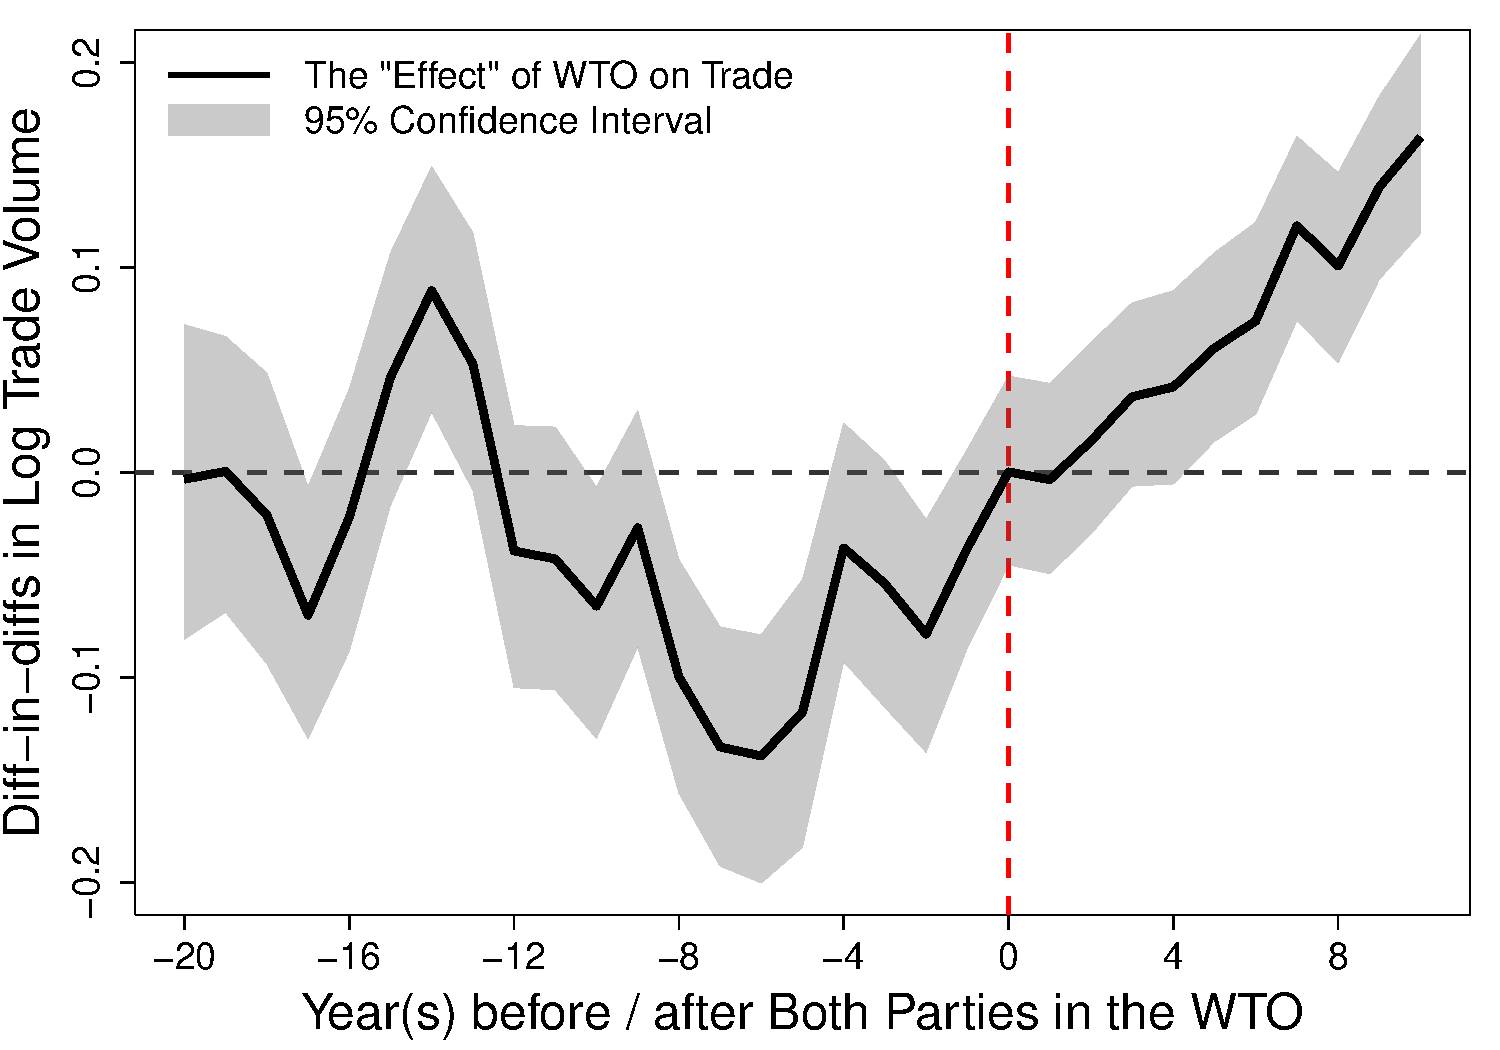
\includegraphics[width=5cm]{ex_trade.pdf}%
\column{.5\textwidth}
\centering
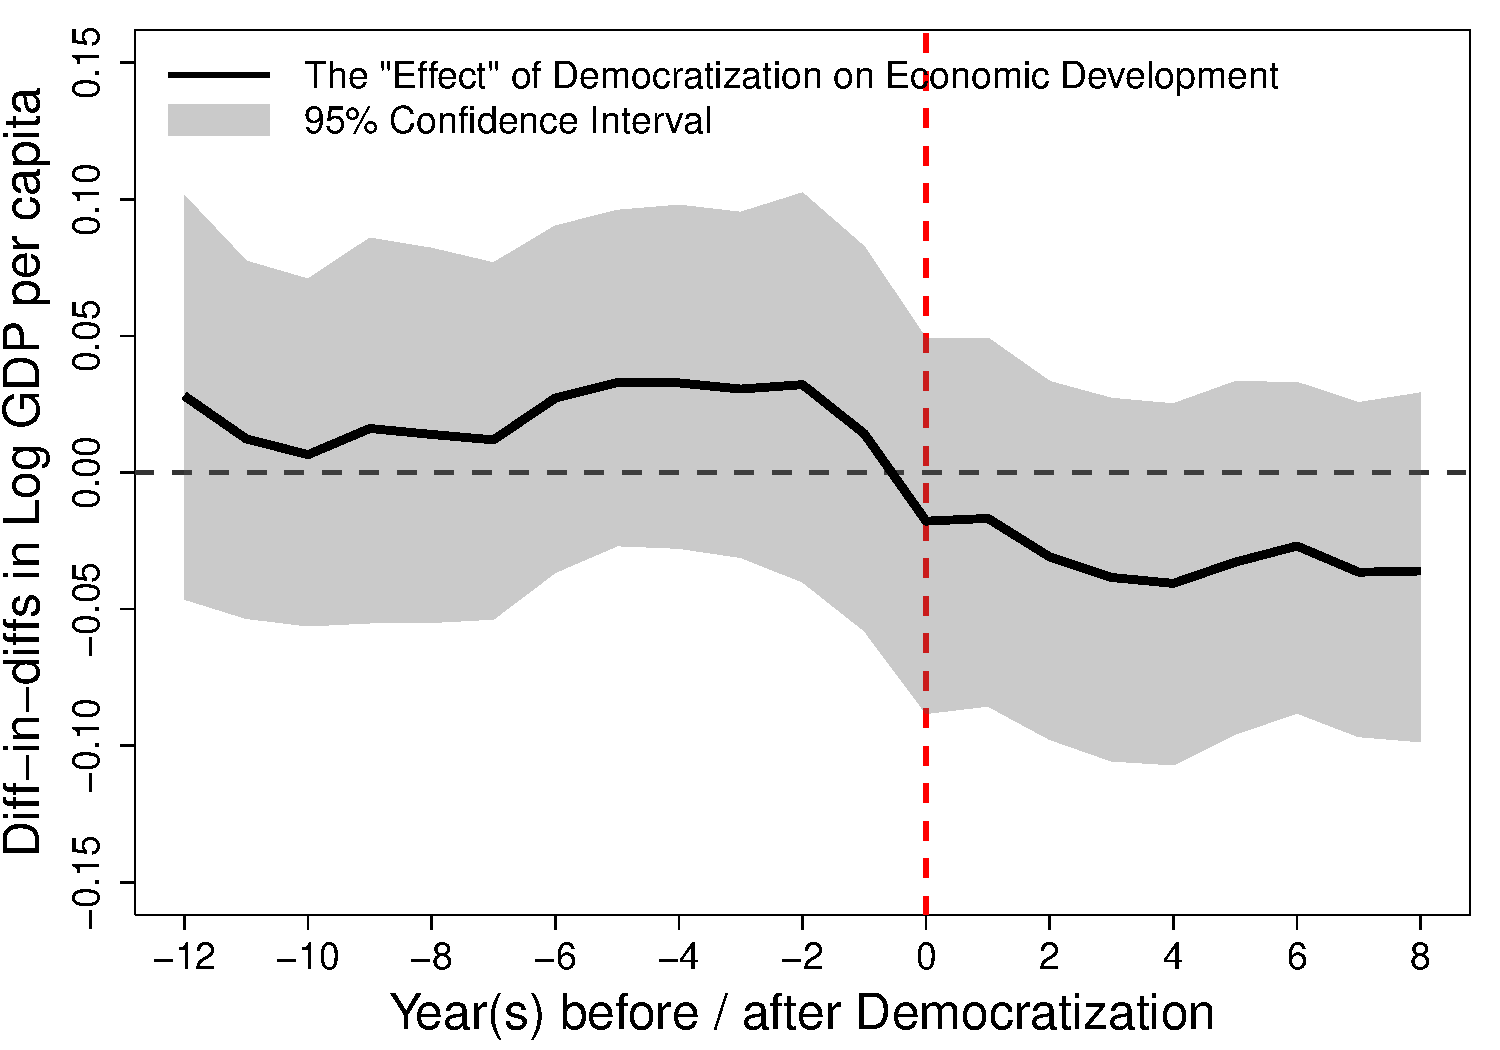
\includegraphics[width=5cm]{ex_demoGDP.pdf}\\\vspace{1em}%
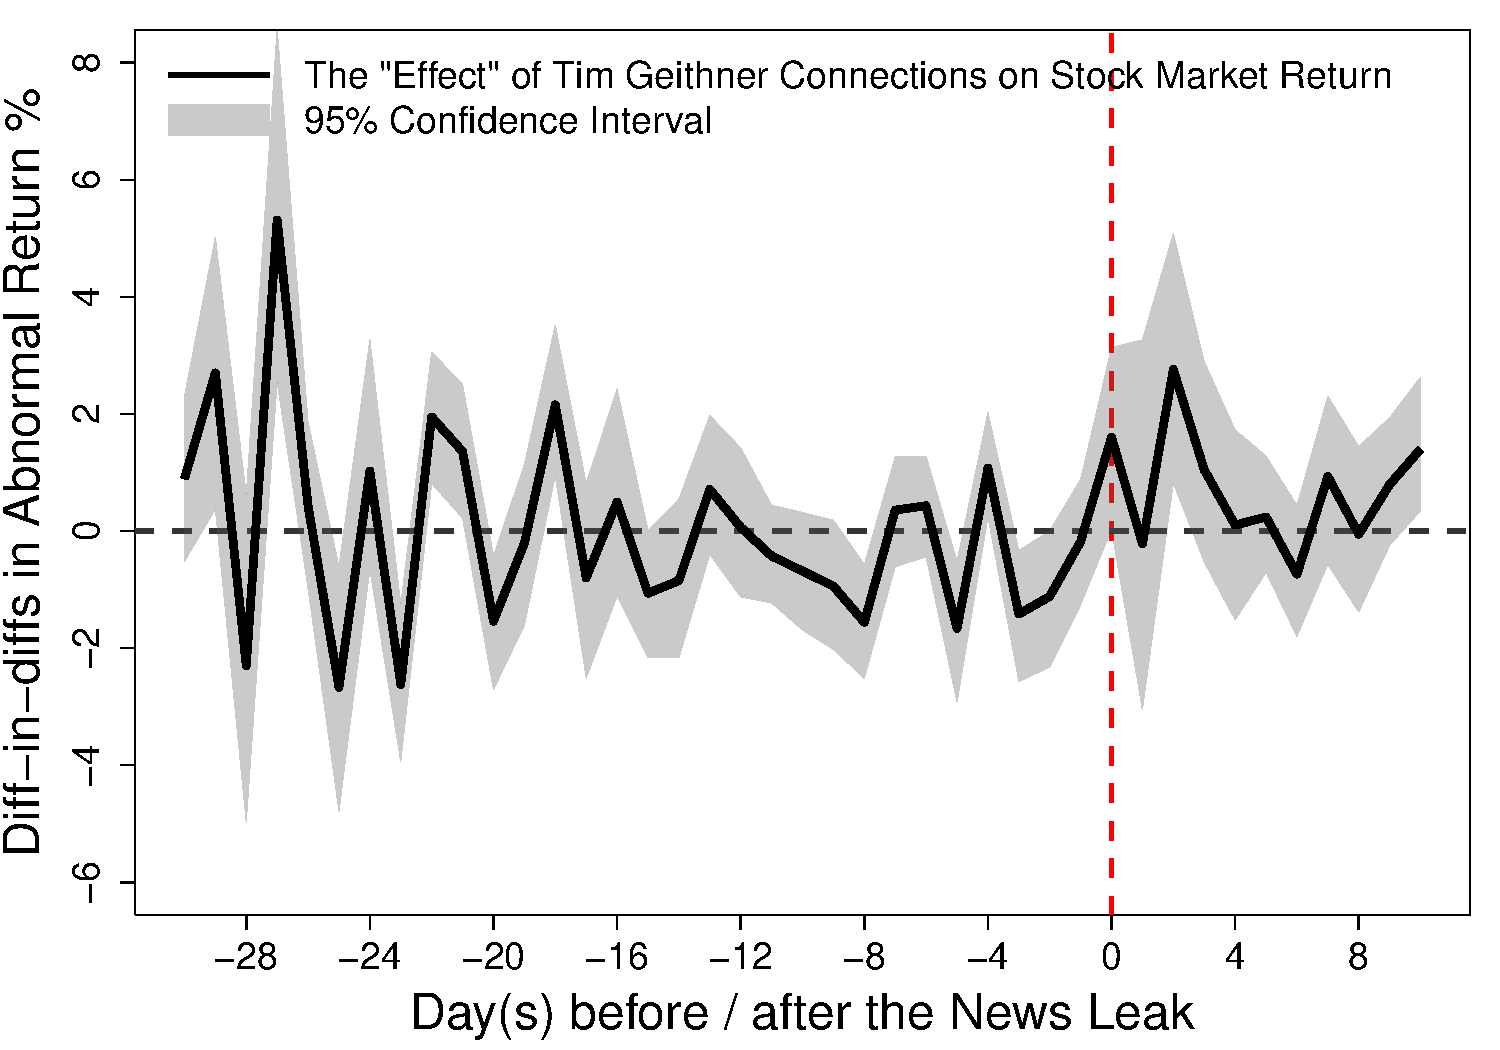
\includegraphics[width=5cm]{ex_ajkkm.pdf}%
\end{columns}
\end{frame}


\if\handout0{
\addtocounter{framenumber}{-1}
\begin{frame}
\frametitle{Signs of Parallel Trends Violations}
\centering\Large
\only<1>{\vspace{1em}\bf Gun Control on Crime\\\vspace{0.8em}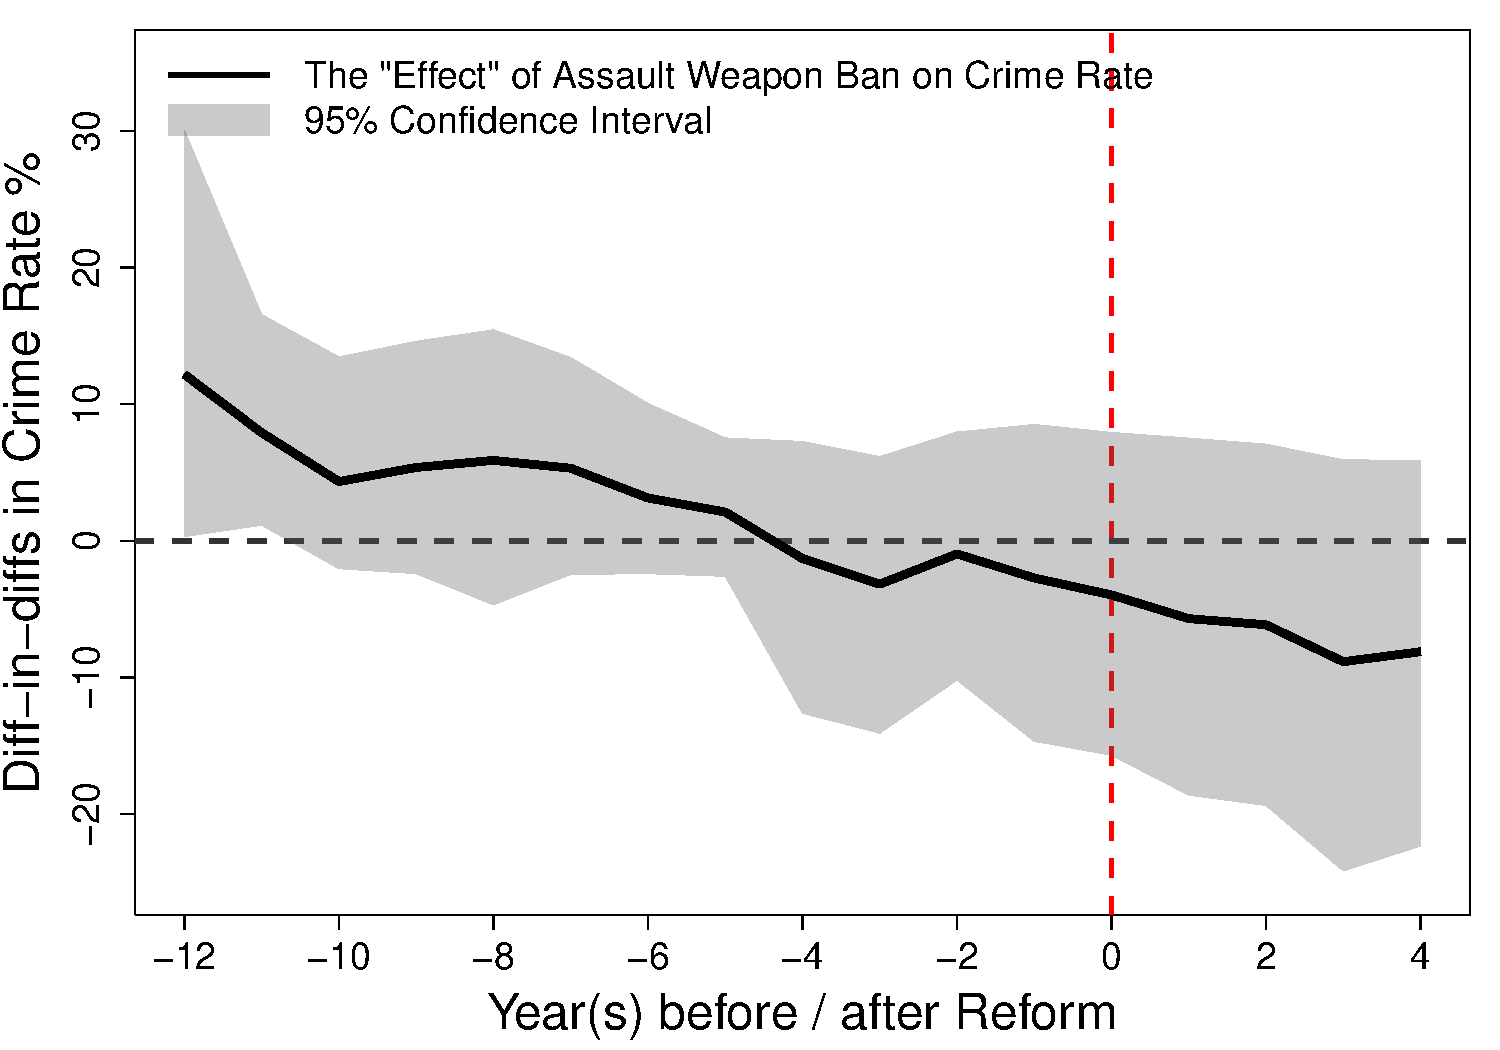
\includegraphics[width=8cm]{ex_guncontrol.pdf}}%
\only<2>{\vspace{1em}\bf Democratization on Development\\\vspace{0.6em}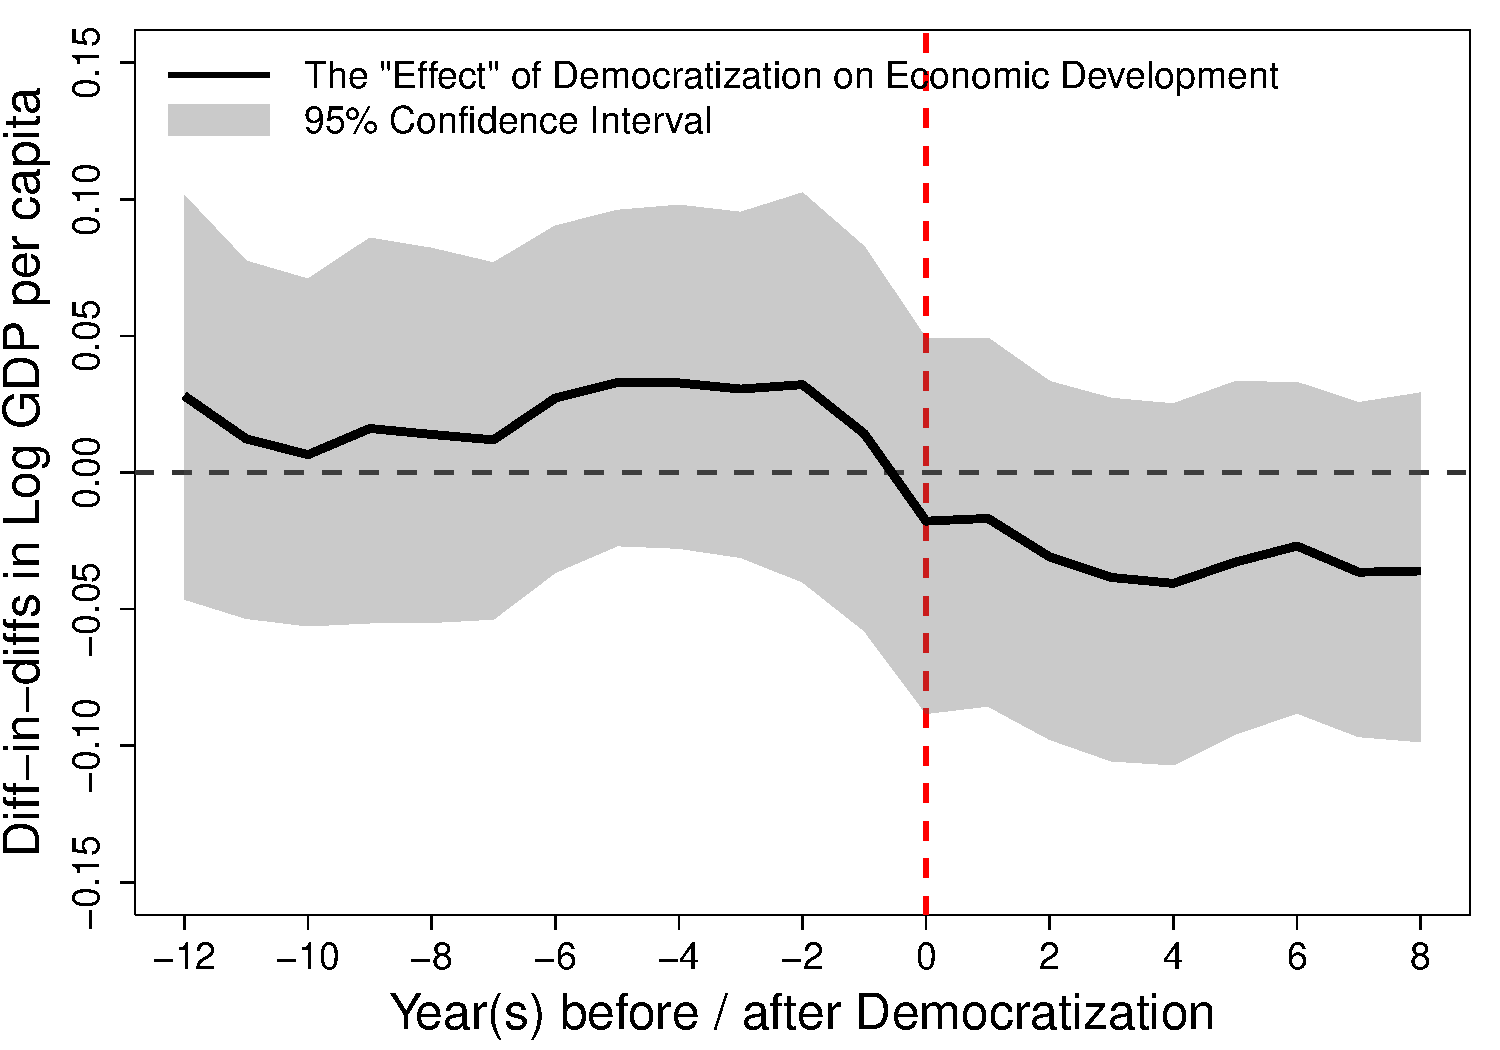
\includegraphics[width=8cm]{ex_demoGDP.pdf}}%
\only<3>{\vspace{1em}\bf WTO on Trade\\\vspace{0.8em}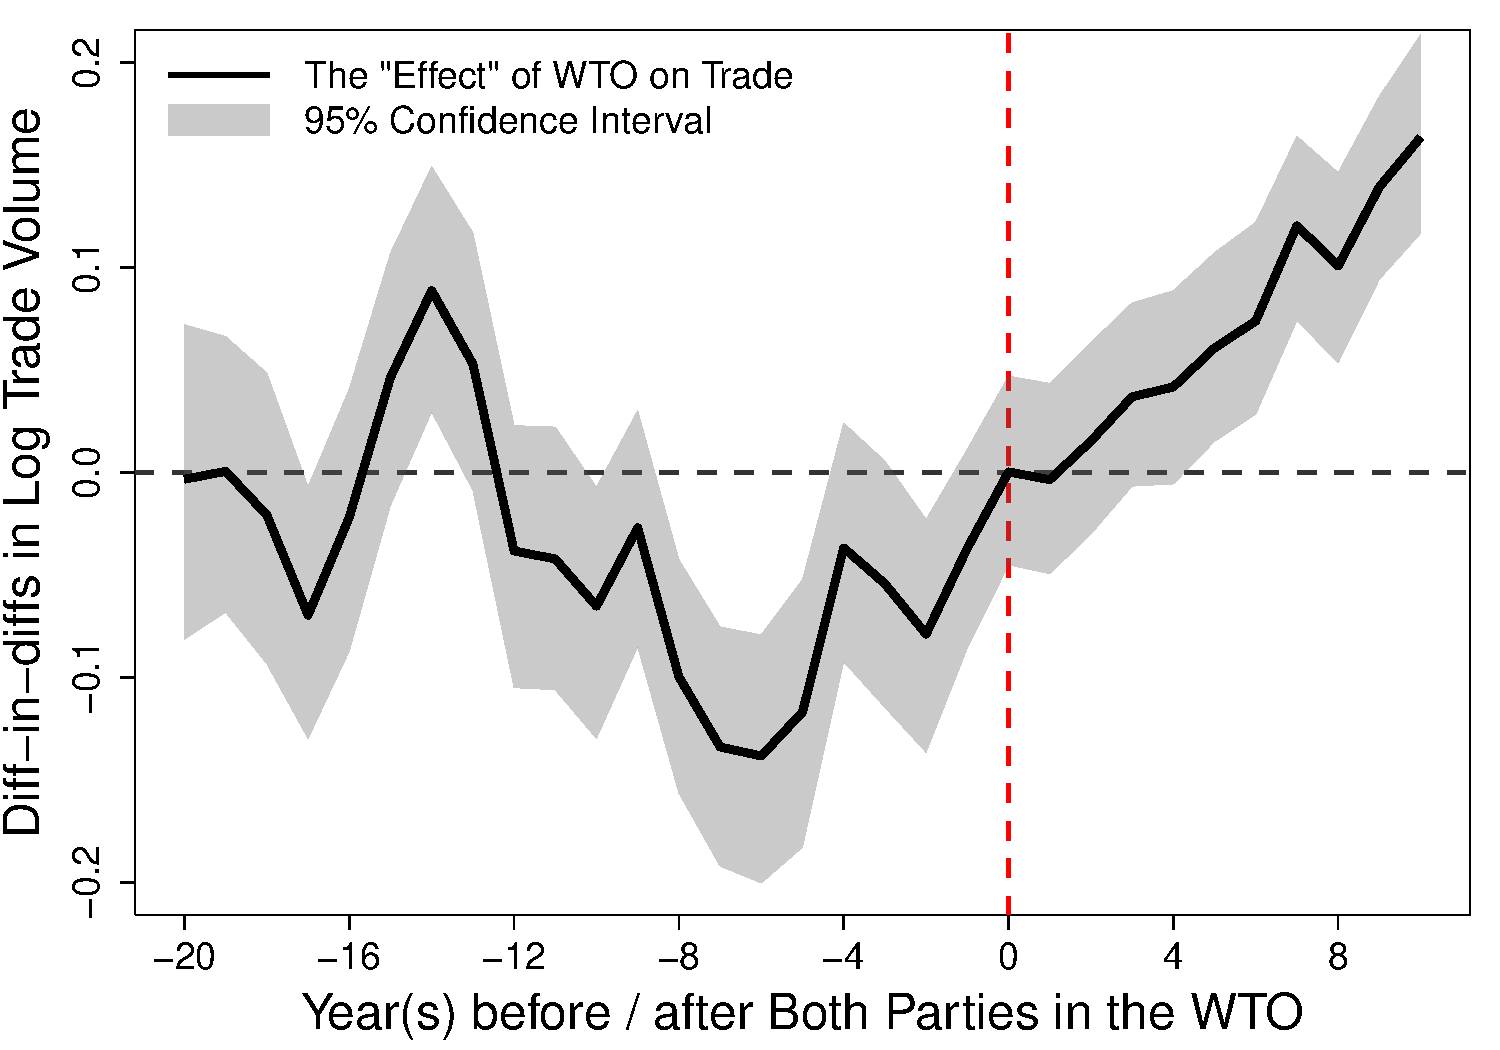
\includegraphics[width=8cm]{ex_trade.pdf}}%
\only<4>{\vspace{1em}\bf Political Connections on Stock Returns\\\vspace{0.8em}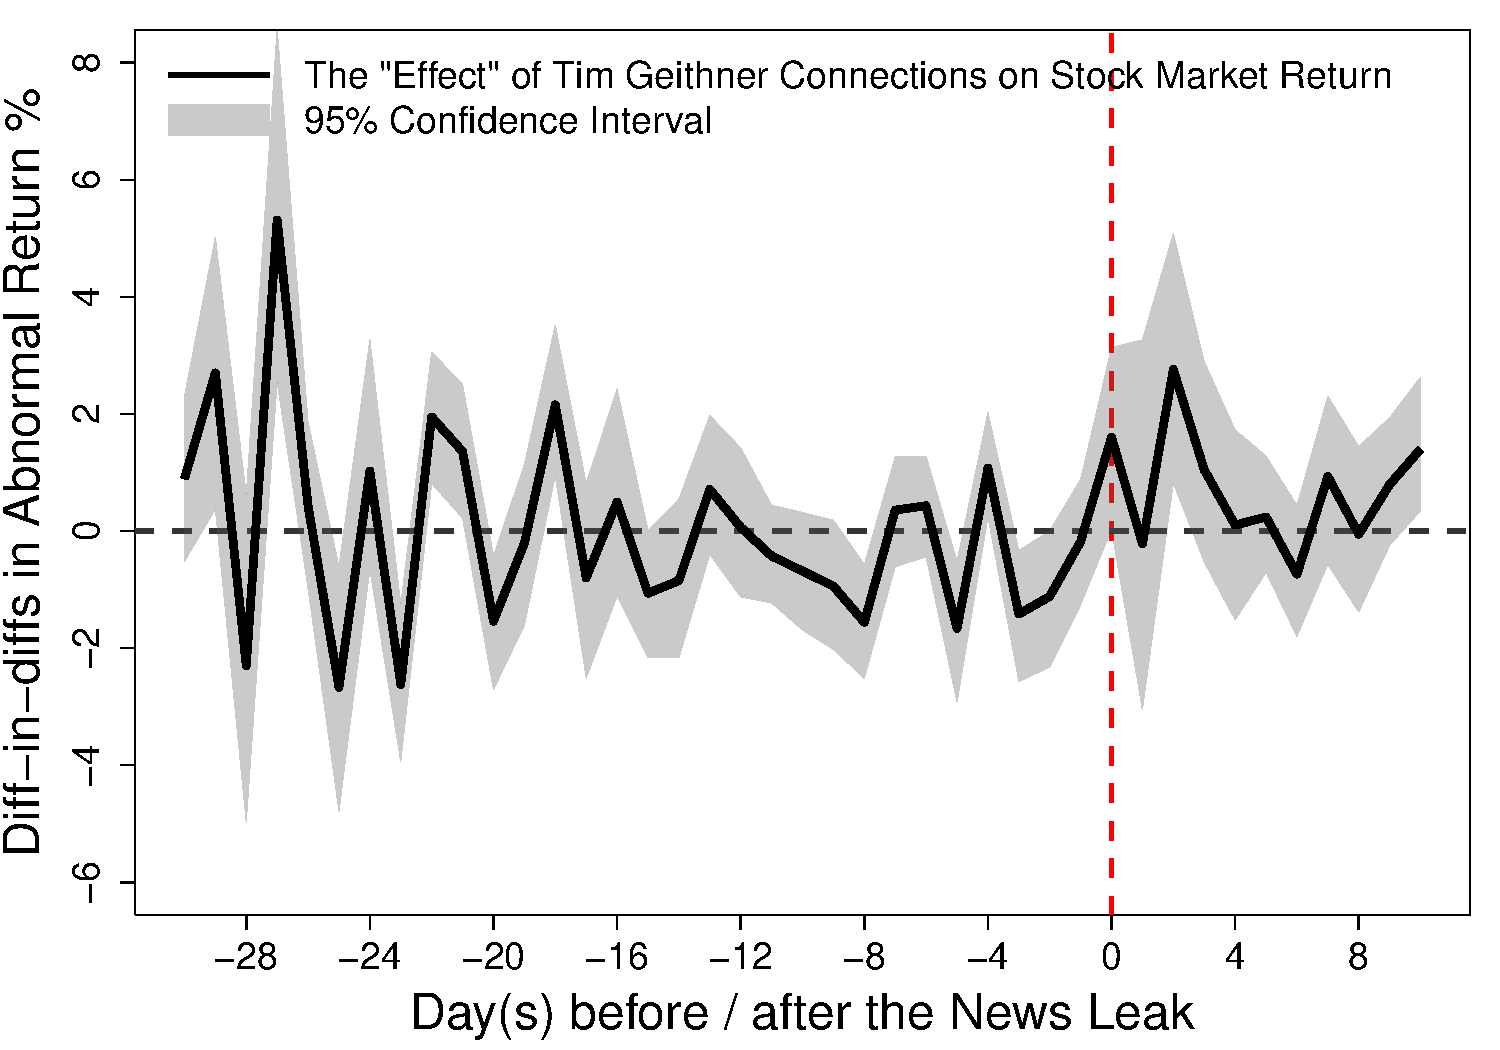
\includegraphics[width=8cm]{ex_ajkkm.pdf}}%
\end{frame}
}
\fi


\begin{frame}
  \frametitle{Simulation: Parallel Trends and Bias}
\begin{center}
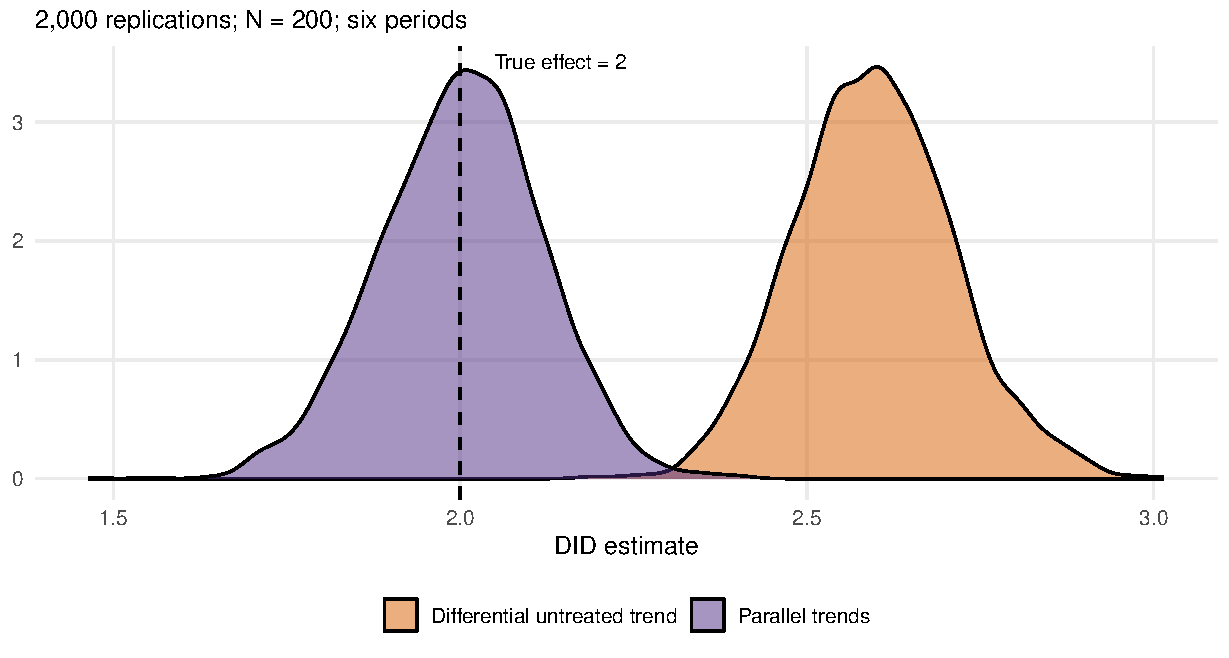
\includegraphics[width=0.80\textwidth]{did_simulation_2026.pdf}
\end{center}
\vspace{-0.8em}
\begin{itemize}
\item When untreated trends are parallel, the estimates center on the true effect.
\item Even a modest differential trend biases DID.
\end{itemize}
\end{frame}


\begin{frame}
  \frametitle{Falsification Test: Alternative Control Group}
\begin{center}{\scriptsize\resizebox{\textwidth}{!}{%
\begin{tabular}{lccc|ccc|cc}
\toprule
& \multicolumn{3}{c|}{Stores by state} & \multicolumn{3}{c|}{Stores in New Jersey, by starting wage} & \multicolumn{2}{c}{Differences within NJ} \\
& PA & NJ & NJ $-$ PA & \$4.25 & \$4.26--4.99 & $\geq$ \$5.00 & Low $-$ high & Mid $-$ high \\ \midrule
FTE employment before & 23.33 (1.35) & 20.44 (0.51) & $-2.89$ (1.44) & 19.56 (0.77) & 20.08 (0.84) & 22.25 (1.14) & $-2.69$ (1.37) & $-2.17$ (1.41) \\
FTE employment after & 21.17 (0.94) & 21.03 (0.52) & $-0.14$ (1.07) & 20.88 (1.01) & 20.96 (0.76) & 20.21 (1.03) & 0.67 (1.44) & 0.75 (1.27) \\
Change in mean FTE employment & $-2.16$ (1.25) & 0.59 (0.54) & 2.76 (1.36) & 1.32 (0.95) & 0.87 (0.84) & $-2.04$ (1.14) & 3.36 (1.48) & 2.91 (1.41) \\
\bottomrule
\end{tabular}}}
\end{center}
{\scriptsize Numbers from \textcite{card1994minimum}, Table 3 (rows 1--3); standard errors in parentheses.}\medskip

If the DID with the alternative control is different from the DID with the original control, then the original DID may be biased% \end{itemize}\medskip \pause
\end{frame}

\if\handout0{
  \begin{frame}
    \frametitle{Triple DID: Mandated Maternity Benefits (\cite{gruber1994incidence})}
  \begin{center}\small
  \begin{tabular}{lccc}
  \toprule
  & Before law change & After law change & Time difference \\ \midrule
  \multicolumn{4}{l}{\emph{A. Treatment individuals: married women, 20--40 years old}} \\
  Experimental states & 1.547 (0.012) & 1.513 (0.012) & $-0.034$ (0.017) \\
  Nonexperimental states & 1.369 (0.010) & 1.397 (0.010) & 0.028 (0.014) \\
  Location difference at a point in time & 0.178 (0.016) & 0.116 (0.015) & \\
  \alert<1>{Difference-in-differences} & & \alert<1>{$-0.062$ (0.022)} & \\ \midrule
  \multicolumn{4}{l}{\uncover<2->{\emph{B. Control group: over 40 and single males, 20--40}}} \\
  \uncover<2->{Experimental states} & \uncover<2->{1.759 (0.007)} & \uncover<2->{1.748 (0.007)} & \uncover<2->{$-0.011$ (0.010)} \\
  \uncover<2->{Nonexperimental states} & \uncover<2->{1.630 (0.007)} & \uncover<2->{1.627 (0.007)} & \uncover<2->{$-0.003$ (0.010)} \\
  \uncover<2->{Location difference at a point in time} & \uncover<2->{0.129 (0.010)} & \uncover<2->{0.121 (0.010)} & \\
  \uncover<2->{\alert<2>{Difference-in-differences}} & & \uncover<2->{\alert<2>{$-0.008$ (0.014)}} & \\ \midrule
  \uncover<3->{\textbf{DDD}} & & \uncover<3->{\alert<3>{$\mathbf{-0.054}$ (0.026)}} & \\
  \bottomrule
  \end{tabular}
  \end{center}
  \slidesource{Log hourly wages; standard errors in parentheses. Numbers from \textcite{gruber1994incidence}, Table 3.}
  \end{frame}
} 
\else {
  \begin{frame}
    \frametitle{Triple DID: Mandated Maternity Benefits (\cite{gruber1994incidence})}
  \begin{center}\small
  \begin{tabular}{lccc}
  \toprule
  & Before law change & After law change & Time difference \\ \midrule
  \multicolumn{4}{l}{\emph{A. Treatment individuals: married women, 20--40 years old}} \\
  Experimental states & 1.547 (0.012) & 1.513 (0.012) & $-0.034$ (0.017) \\
  Nonexperimental states & 1.369 (0.010) & 1.397 (0.010) & 0.028 (0.014) \\
  Location difference at a point in time & 0.178 (0.016) & 0.116 (0.015) & \\
  Difference-in-differences & & $-0.062$ (0.022) & \\ \midrule
  \multicolumn{4}{l}{\emph{B. Control group: over 40 and single males, 20--40}} \\
  Experimental states & 1.759 (0.007) & 1.748 (0.007) & $-0.011$ (0.010) \\
  Nonexperimental states & 1.630 (0.007) & 1.627 (0.007) & $-0.003$ (0.010) \\
  Location difference at a point in time & 0.129 (0.010) & 0.121 (0.010) & \\
  Difference-in-differences & & $-0.008$ (0.014) & \\ \midrule
  \textbf{DDD} & & $\mathbf{-0.054}$ (0.026) & \\
  \bottomrule
  \end{tabular}
  \end{center}
  \slidesource{Log hourly wages; standard errors in parentheses. Numbers from \textcite{gruber1994incidence}, Table 3.}
  \end{frame}  
}\fi

\begin{frame}
  \frametitle{How Useful is Triple DID?}
\begin{itemize}
  \item The triple DID estimate is the difference between the DID of interest and the placebo DID (that is supposed to be zero)\bigskip
  \begin{itemize}
\item If the placebo DID is nonzero, it might be difficult to convince reviewers
that the triple DID removes all the bias\medskip
    \item If the placebo DID is zero, then DID and triple DID give the same results but DID is preferable because standard errors are smaller for DD than for triple DID
  \end{itemize}
\end{itemize}
\end{frame}

 
\begin{frame}
  \frametitle{Compositional Differences}

\begin{itemize}[<+->]\itemsep1em
  \item In repeated cross-sections, we do not want that the composition of the sample changes between periods.\medskip
\item Examples:
\begin{itemize}\itemsep0.5em
  \item \textcite{hong2013measuring} uses repeated cross-sectional data from Consumer Expenditure Survey (CEX) containing music expenditures and internet use for random samples of U.S. households\medskip
   \item Study exploits the emergence of Napster (the first sharing software widely used by Internet users) in June 1999 as a natural experiment.\medskip
  \item Study compares internet users and internet non-users, before and after emergence of Napster
\end{itemize}
\end{itemize}
\end{frame}

\begin{frame}
  \frametitle{Compositional Differences?}
\begin{center}
{\small Effect of Napster on quarterly music spending (1998 dollars)}\par\medskip
\begin{tabular}{lcc}
\toprule
& Age 15--34 & Households with children aged 6--17 \\ \midrule
\multicolumn{3}{l}{\emph{A. DD estimate}} \\
$\theta$ & $-3.432$ (1.284) & $-3.258$ (1.203) \\ \midrule
\multicolumn{3}{l}{\emph{B. 2SIV estimates}} \\
$\theta_0$ & $-2.427$ (0.949) & $-0.120$ (1.092) \\
$\theta_1$ & $-2.719$ (2.079) & $-22.510$ (6.889) \\
Mean imputed downloading probability & 0.346 & 0.140 \\
\bottomrule
\end{tabular}
\end{center}
\medskip
\begin{itemize}
\item<2-> The DD estimate compares internet users with non-users before and after Napster; the 2SIV step lets the effect differ by the imputed probability of downloading
\end{itemize}
\slidesource{Numbers from \textcite{hong2013measuring}, Table 8; standard errors in parentheses.}
\end{frame}

\begin{frame}
  \frametitle{Compositional Differences?}
\begin{center}{\small
\begin{tabular}{lcccccccc}
\toprule
& \multicolumn{2}{c}{1997} & \multicolumn{2}{c}{1998} & \multicolumn{2}{c}{1999} & \multicolumn{2}{c}{2000} \\
& Users & Non & Users & Non & Users & Non & Users & Non \\ \midrule
Recorded music spending (\$) & 25.73 & 10.90 & 24.18 & 9.97 & 20.92 & 9.37 & 17.42 & 8.22 \\
Age & 40.2 & 49.0 & 42.3 & 49.0 & 44.1 & 49.4 & 44.3 & 49.9 \\
Income (\$) & 52,887 & 30,459 & 51,995 & 28,169 & 49,970 & 26,649 & 47,510 & 26,336 \\
College graduate & .43 & .21 & .45 & .21 & .42 & .20 & .37 & .20 \\
Owns a computer & .79 & .27 & .81 & .28 & .80 & .28 & .81 & .32 \\
Households (millions) & 15 & 91 & 22 & 86 & 28 & 80 & 34 & 76 \\
\bottomrule
\end{tabular}}
\end{center}
\medskip
Diffusion of the internet changes the samples: the early adopters were younger, richer music fans; later users look more like everyone else
\slidesource{Internet users and non-users in the Consumer Expenditure Survey; numbers from \textcite{hong2013measuring}, Table 1.}

\end{frame}

\begin{frame}
  \frametitle{Long-term Effects versus Reliability}
\begin{columns}[c]  
\column{.4\textwidth}
\begin{itemize}\medskip
  \item Parallel trends assumption for DID is more likely to hold over
a shorter time-window\medskip
\item In the long-run, many other things may happen that could confound the effect of the treatment\medskip
\item Should be cautious to extrapolate short-term effects to long-term effects
\end{itemize}\pause
\column{.6\textwidth}
Effect of War on Tax Rates \parencite{scheve2010conscription}  
\begin{center}
  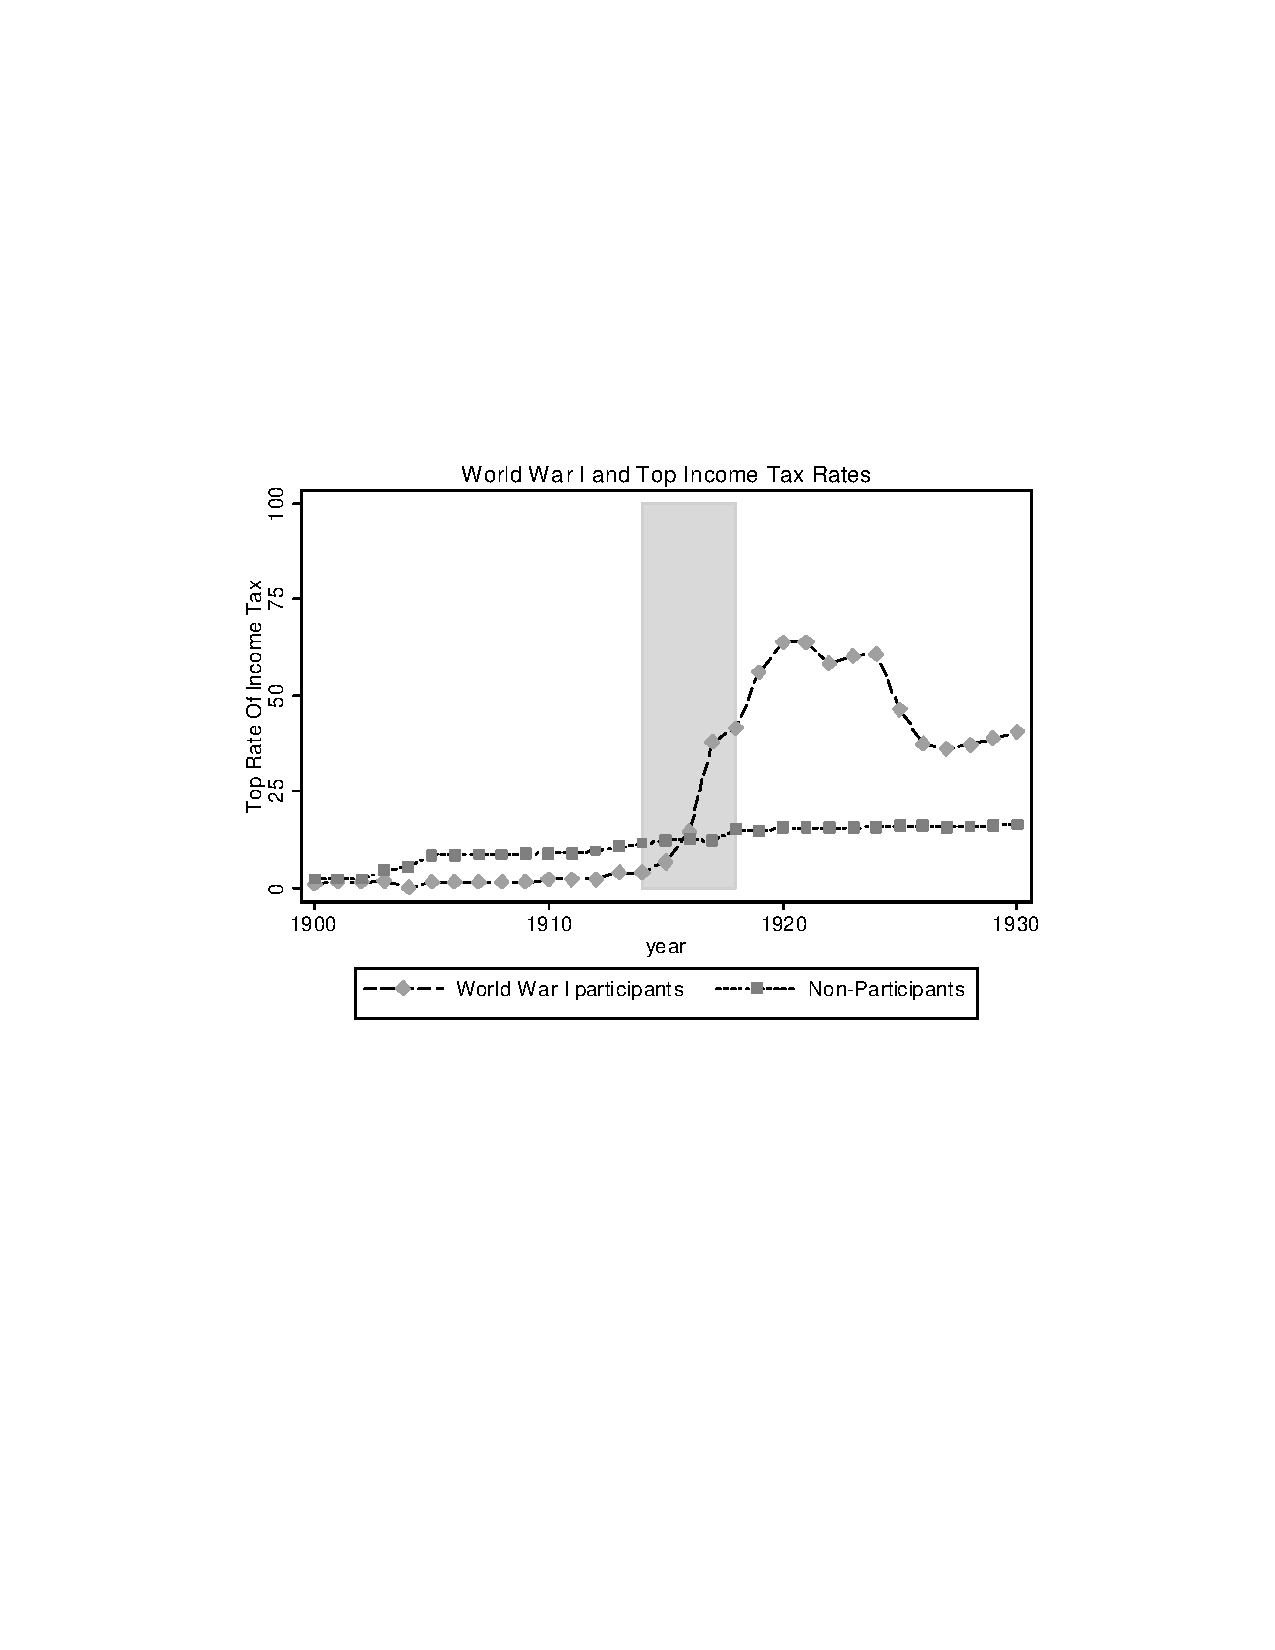
\includegraphics[height=1.8in,keepaspectratio=1]{Ken.pdf}
\end{center}  \vspace{-.0in}
\end{columns}
\slidesource{Figure 1 of \textcite{scheve2010conscription}, reproduced with attribution: top marginal income tax rates, World War I participants vs.\ non-participants.}
\end{frame}


\begin{frame}
  \frametitle{Scale Dependence}
Magnitude or even sign of the DID effect may be sensitive to the functional form, when average outcomes for controls and treated are very different at baseline
 \begin{itemize}\bigskip
 \item Training program for the young:\medskip
 \begin{itemize}
   \item Employment for the young increases from 20\% to 30\%
   \item Employment for the old increases from 5\% to 10\%
   \item Positive DID effect: $(30 - 20) - (10 - 5) = 5\%$ increase\medskip \pause
   \item But if you consider log changes in employment, the DD is,
$[log(30) - log(20)] - [log(10) - log(5)] = log(1.5)- log(2) < 0$
 \end{itemize}\bigskip
 \item DD estimates may be more reliable if treated and controls are more similar at baseline\medskip
 \item More similarity may help with parallel trends assumption
\end{itemize}
\end{frame}

\begin{frame}
  \frametitle{When the Parallel Trends Assumption is More Defensible?}
  \alert{\textcite{roth2023when}}
  \begin{itemize}[<+->]\itemsep1em
    \item The parallel trends assumption is scale-dependent
    \item When is the assumption not sensitive to strictly monotonic transformation of the outcome? 
    \item A ``stronger parallel trends'' for the entire distribution of $Y_{it}(0)$
    $$F^{Y(0)}_{G=1,t=1}(y) - F^{Y(0)}_{G=1,t=0}(y) = F^{Y(0)}_{G=0,t=1}(y) - F^{Y(0)}_{G=0,t=0}(y),\qquad \text{ for all } y \in \mathcal{R}$$
    \item It holds when the population are consists of\medskip
    \begin{itemize}\itemsep0.5em
      \item A subgroup in which the treatment is as-if randomly assigned
      \item A subgroup in which the distribution of $Y_{it}(0)$ is stable over time
    \end{itemize}
  \end{itemize}
  \end{frame}


%\end{frame}


%\end{frame}


%\end{frame}


\begin{frame}[t]{Conclusion}
\begin{itemize}[<+->]\itemsep1em
\item DID is a powerful research design for causal inference with
panel or repeated cross-sectional data
\item The parallel trends assumption embeds a functional form requirement, which
is \red{scale dependent}
\item Researchers should be concerned about its validity and use various
falsification tests to probe its plausibility
\end{itemize}
\end{frame}


\appendix

\setbeamertemplate{frametitle continuation}[from second][(cont.)]
\begin{frame}[t,allowframebreaks=1.0]
  \frametitle{References}
  \referencelist
  \vfill{\footnotesize\color{gray}Parts of this lecture build on teaching slides by Jens Hainmueller.}
\end{frame}

\end{document}
